\pdfbookmark{Общая характеристика работы}{characteristic}             % Закладка pdf
\section*{Общая характеристика работы}

\newcommand{\actuality}{\pdfbookmark[1]{Актуальность}{actuality}\underline{\textbf{\actualityTXT}}}
\newcommand{\progress}{\pdfbookmark[1]{Разработанность темы}{progress}\underline{\textbf{\progressTXT}}}
\newcommand{\aim}{\pdfbookmark[1]{Цели}{aim}\underline{{\textbf\aimTXT}}}
\newcommand{\tasks}{\pdfbookmark[1]{Задачи}{tasks}\underline{\textbf{\tasksTXT}}}
\newcommand{\aimtasks}{\pdfbookmark[1]{Цели и задачи}{aimtasks}\aimtasksTXT}
\newcommand{\researchObject}{\pdfbookmark[1]{Объект исследования}{researchObject}\underline{\textbf{\researchObjectTXT}}}
\newcommand{\researchSubject}{\pdfbookmark[1]{Субъект исследования}{researchSubject}\underline{\textbf{\researchSubjectTXT}}}
\newcommand{\novelty}{\pdfbookmark[1]{Научная новизна}{novelty}\underline{\textbf{\noveltyTXT}}}
\newcommand{\theoreticalValue}{\pdfbookmark[1]{Теоретическая значимость}{theoreticalValue}\underline{\textbf{\theoreticalValueTXT}}}
\newcommand{\practicalValue}{\pdfbookmark[1]{Практическая значимость}{practicalValue}\underline{\textbf{\practicalValueTXT}}}
\newcommand{\influence}{\pdfbookmark[1]{Практическая значимость}{influence}\underline{\textbf{\influenceTXT}}}
\newcommand{\methods}{\pdfbookmark[1]{Методология и методы исследования}{methods}\underline{\textbf{\methodsTXT}}}
\newcommand{\defpositions}{\pdfbookmark[1]{Положения, выносимые на защиту}{defpositions}\underline{\textbf{\defpositionsTXT}}}
\newcommand{\reliability}{\pdfbookmark[1]{Достоверность}{reliability}\underline{\textbf{\reliabilityTXT}}}
\newcommand{\probation}{\pdfbookmark[1]{Апробация}{probation}\underline{\textbf{\probationTXT}}}
\newcommand{\contribution}{\pdfbookmark[1]{Личный вклад}{contribution}\underline{\textbf{\contributionTXT}}}
\newcommand{\publications}{\pdfbookmark[1]{Публикации}{publications}\underline{\textbf{\publicationsTXT}}}


{\actuality} Обзор, введение в тему, обозначение места данной работы в
мировых исследованиях и~т.\:п., можно использовать ссылки на~другие
работы~\autocite{Gosele1999161,Lermontov}
(если их~нет, то~в~автореферате
автоматически пропадёт раздел <<Список литературы>>). Внимание! Ссылки
на~другие работы в~разделе общей характеристики работы можно
использовать только при использовании \verb!biblatex! (из-за технических
ограничений \verb!bibtex8!. Это связано с тем, что одна
и~та~же~характеристика используются и~в~тексте диссертации, и в
автореферате. В~последнем, согласно ГОСТ, должен присутствовать список
работ автора по~теме диссертации, а~\verb!bibtex8! не~умеет выводить в~одном
файле два списка литературы).
При использовании \verb!biblatex! возможно использование исключительно
в~автореферате подстрочных ссылок
для других работ командой \verb!\autocite!~\autocite{Marketing}, а~также цитирование
собственных работ командой \verb!\cite!. Для этого в~файле
\verb!common/setup.tex! необходимо присвоить положительное значение
счётчику \verb!\setcounter{usefootcite}{1}!.

Для генерации содержимого титульного листа автореферата, диссертации
и~презентации используются данные из файла \verb!common/data.tex!. Если,
например, вы меняете название диссертации, то оно автоматически
появится в~итоговых файлах после очередного запуска \LaTeX. Согласно
ГОСТ 7.0.11-2011 <<5.1.1 Титульный лист является первой страницей
диссертации, служит источником информации, необходимой для обработки и
поиска документа>>. Наличие логотипа организации на~титульном листе
упрощает обработку и~поиск, для этого разметите логотип вашей
организации в папке images в~формате PDF (лучше найти его в векторном
варианте, чтобы он хорошо смотрелся при печати) под именем
\verb!logo.pdf!. Настроить размер изображения с логотипом можно
в~соответствующих местах файлов \verb!title.tex!  отдельно для
диссертации и автореферата. Если вам логотип не~нужен, то просто
удалите файл с~логотипом.

\ifsynopsis
Этот абзац появляется только в~автореферате.
Для формирования блоков, которые будут обрабатываться только в~автореферате,
заведена проверка условия \verb!\!\verb!ifsynopsis!.
Значение условия задаётся в~основном файле документа (\verb!synopsis.tex! для
автореферата).
\else
Этот абзац появляется только в~диссертации.
Через проверку условия \verb!\!\verb!ifsynopsis!, задаваемого в~основном файле
документа (\verb!dissertation.tex! для диссертации), можно сделать новую
команду, обеспечивающую появление цитаты в~диссертации, но~не~в~автореферате.
\fi

% {\progress}
% Этот раздел должен быть отдельным структурным элементом по
% ГОСТ, но он, как правило, включается в описание актуальности
% темы. Нужен он отдельным структурынм элемементом или нет ---
% смотрите другие диссертации вашего совета, скорее всего не нужен.

{\aim} данной работы является повышение эффективности анализа неопределенных данных путем разработки математического и программного обеспечения на основе мягких вычислений.

Для~достижения поставленной цели необходимо было решить следующие {\tasks}:
\begin{enumerate}[beginpenalty=10000] % https://tex.stackexchange.com/a/476052/104425
  \item Провести обзор проблем и предлагаемых подходов построения нечетких систем анализа данных с качественным описанием.
  \item Разработать метод вывода на основое нечеткого значения истинности для системы MISO-сструктуры логического типа, обеспечивающий полиномиальную вычислительную сложность.
  \item Выполнить программную реализацию выработанного метода нечеткого вывода с использованием технологии параллельных вычислений CUDA, обеспечив эффективность реализации за счет внедрения оптимизаций алгоритма вывода.
  \item Применить разработанный модуль нечеткого логического вывода для высокопроизводительного анализа зашумленных данных в выбранной предметной области.
\end{enumerate}


{\novelty}
\begin{enumerate}[beginpenalty=10000] % https://tex.stackexchange.com/a/476052/104425
  \item Впервые применено нечеткое значение истинности и принцип обобщения для получения выходного значения при нескольких нечетких входах в соответствии с обобщенным нечетким правилом вывода \textit{modus ponens} для нечетких систем логического типа, в результате чего была получена новая структура базы правил: <<Если \textit{истинно}, то $B_k$>>.
  \item Разработан метод нечеткого вывода логического типа с использованием нечеткого значения истинности, имеющий полиномиальную вычислительную сложность при многих нечетких входах.
  \item Разработан метод регрессии временных рядов с нечеткими оценками измеренных значений на основе предложенного метода нечеткого вывода логического типа и алгоритм построения базы правил \dots.
  \item Разработан параллельный алгоритм, реализующий нечеткий вывод на основе нечеткого значения истинности с применением отбора \dots
\end{enumerate}

{\influence} \ldots

{\methods} \ldots

{\defpositions}
\begin{enumerate}[beginpenalty=10000] % https://tex.stackexchange.com/a/476052/104425
  \item Метод вывода для нечетких систем логического типа на основе нечеткого значения истинности, имеющий полиномиальную вычислительную сложность при многих нечетких входах.
  \item Метод регрессии для временных рядов с нечеткими оценками измеренных значений на основе метода нечеткого вывода логического типа.
  \item Разработанный вид нечетких правил <<Если \textit{истинно}, то $B_k$>>.
  \item Разработанный параллельный алгоритм для предложенного метода вывода и его эффективная реализация на графическом процессоре с поддержкой технологии CUDA.
  \item \dots
  \item \dots
\end{enumerate}
В папке Documents можно ознакомиться с решением совета из Томского~ГУ
(в~файле \verb+Def_positions.pdf+), где обоснованно даются рекомендации
по~формулировкам защищаемых положений.

\textbf{Соответствие диссертации научной специальности.} Диссертационная работа соответствует паспорту специальности 2.3.1. <<Системный анализ, управление и обработка информации, статистика>> по следующим областям исследования:
\begin{itemize}
  \item п. 10 <<Методы и алгоритмы интеллектуальной поддержки при принятии управленческих решений в технических системах>>.
\end{itemize}


{\reliability} полученных результатов обеспечивается \ldots \ Результаты находятся в соответствии с результатами, полученными другими авторами.

{\probation}
Основные результаты работы докладывались~на:
перечисление основных конференций, симпозиумов и~т.\:п.

{\contribution} Все изложенные в диссертации результаты исследования получены либо соискателем лично, либо при его непосредственном участии.

\ifnumequal{\value{bibliosel}}{0}
{%%% Встроенная реализация с загрузкой файла через движок bibtex8. (При желании, внутри можно использовать обычные ссылки, наподобие `\cite{vakbib1,vakbib2}`).
    {\publications} Основные результаты по теме диссертации изложены
    в~XX~печатных изданиях,
    X из которых изданы в журналах, рекомендованных ВАК,
    X "--- в тезисах докладов.
}%
{%%% Реализация пакетом biblatex через движок biber
    \begin{refsection}[bl-author, bl-registered]
        % Это refsection=1.
        % Процитированные здесь работы:
        %  * подсчитываются, для автоматического составления фразы "Основные результаты ..."
        %  * попадают в авторскую библиографию, при usefootcite==0 и стиле `\insertbiblioauthor` или `\insertbiblioauthorgrouped`
        %  * нумеруются там в зависимости от порядка команд `\printbibliography` в этом разделе.
        %  * при использовании `\insertbiblioauthorgrouped`, порядок команд `\printbibliography` в нём должен быть тем же (см. biblio/biblatex.tex)
        %
        % Невидимый библиографический список для подсчёта количества публикаций:
        \phantom{\printbibliography[heading=nobibheading, section=1, env=countauthorvak,          keyword=biblioauthorvak]%
        \printbibliography[heading=nobibheading, section=1, env=countauthorwos,          keyword=biblioauthorwos]%
        \printbibliography[heading=nobibheading, section=1, env=countauthorscopus,       keyword=biblioauthorscopus]%
        \printbibliography[heading=nobibheading, section=1, env=countauthorconf,         keyword=biblioauthorconf]%
        \printbibliography[heading=nobibheading, section=1, env=countauthorother,        keyword=biblioauthorother]%
        \printbibliography[heading=nobibheading, section=1, env=countregistered,         keyword=biblioregistered]%
        \printbibliography[heading=nobibheading, section=1, env=countauthorpatent,       keyword=biblioauthorpatent]%
        \printbibliography[heading=nobibheading, section=1, env=countauthorprogram,      keyword=biblioauthorprogram]%
        \printbibliography[heading=nobibheading, section=1, env=countauthor,             keyword=biblioauthor]%
        \printbibliography[heading=nobibheading, section=1, env=countauthorvakscopuswos, filter=vakscopuswos]%
        \printbibliography[heading=nobibheading, section=1, env=countauthorscopuswos,    filter=scopuswos]}%
        %
        \nocite{*}%
        %
        {\publications} Основные результаты по теме диссертации изложены в~\arabic{citeauthor}~печатных изданиях,
        \arabic{citeauthorvak} из которых изданы в журналах, рекомендованных ВАК%
        \ifnum \value{citeauthorscopuswos}>0%
            , \arabic{citeauthorscopuswos} "--- в~периодических научных журналах, индексируемых Web of~Science и Scopus%
        \fi%
        \ifnum \value{citeauthorconf}>0%
            , \arabic{citeauthorconf} "--- в~тезисах докладов.
        \else%
            .
        \fi%
        \ifnum \value{citeregistered}=1%
            \ifnum \value{citeauthorpatent}=1%
                Зарегистрирован \arabic{citeauthorpatent} патент.
            \fi%
            \ifnum \value{citeauthorprogram}=1%
                Зарегистрирована \arabic{citeauthorprogram} программа для ЭВМ.
            \fi%
        \fi%
        \ifnum \value{citeregistered}>1%
            Зарегистрированы\ %
            \ifnum \value{citeauthorpatent}>0%
            \formbytotal{citeauthorpatent}{патент}{}{а}{}%
            \ifnum \value{citeauthorprogram}=0 . \else \ и~\fi%
            \fi%
            \ifnum \value{citeauthorprogram}>0%
            \formbytotal{citeauthorprogram}{программ}{а}{ы}{} для ЭВМ.
            \fi%
        \fi%
        % К публикациям, в которых излагаются основные научные результаты диссертации на соискание учёной
        % степени, в рецензируемых изданиях приравниваются патенты на изобретения, патенты (свидетельства) на
        % полезную модель, патенты на промышленный образец, патенты на селекционные достижения, свидетельства
        % на программу для электронных вычислительных машин, базу данных, топологию интегральных микросхем,
        % зарегистрированные в установленном порядке.(в ред. Постановления Правительства РФ от 21.04.2016 N 335)
    \end{refsection}%
    \begin{refsection}[bl-author, bl-registered]
        % Это refsection=2.
        % Процитированные здесь работы:
        %  * попадают в авторскую библиографию, при usefootcite==0 и стиле `\insertbiblioauthorimportant`.
        %  * ни на что не влияют в противном случае
        \nocite{vakbib2}%vak
        \nocite{patbib1}%patent
        \nocite{progbib1}%program
        \nocite{bib1}%other
        \nocite{confbib1}%conf
    \end{refsection}%
        %
        % Всё, что вне этих двух refsection, это refsection=0,
        %  * для диссертации - это нормальные ссылки, попадающие в обычную библиографию
        %  * для автореферата:
        %     * при usefootcite==0, ссылка корректно сработает только для источника из `external.bib`. Для своих работ --- напечатает "[0]" (и даже Warning не вылезет).
        %     * при usefootcite==1, ссылка сработает нормально. В авторской библиографии будут только процитированные в refsection=0 работы.
}

При использовании пакета \verb!biblatex! будут подсчитаны все работы, добавленные
в файл \verb!biblio/author.bib!. Для правильного подсчёта работ в~различных
системах цитирования требуется использовать поля:
\begin{itemize}
        \item \texttt{authorvak} если публикация индексирована ВАК,
        \item \texttt{authorscopus} если публикация индексирована Scopus,
        \item \texttt{authorwos} если публикация индексирована Web of Science,
        \item \texttt{authorconf} для докладов конференций,
        \item \texttt{authorpatent} для патентов,
        \item \texttt{authorprogram} для зарегистрированных программ для ЭВМ,
        \item \texttt{authorother} для других публикаций.
\end{itemize}
Для подсчёта используются счётчики:
\begin{itemize}
        \item \texttt{citeauthorvak} для работ, индексируемых ВАК,
        \item \texttt{citeauthorscopus} для работ, индексируемых Scopus,
        \item \texttt{citeauthorwos} для работ, индексируемых Web of Science,
        \item \texttt{citeauthorvakscopuswos} для работ, индексируемых одной из трёх баз,
        \item \texttt{citeauthorscopuswos} для работ, индексируемых Scopus или Web of~Science,
        \item \texttt{citeauthorconf} для докладов на конференциях,
        \item \texttt{citeauthorother} для остальных работ,
        \item \texttt{citeauthorpatent} для патентов,
        \item \texttt{citeauthorprogram} для зарегистрированных программ для ЭВМ,
        \item \texttt{citeauthor} для суммарного количества работ.
\end{itemize}
% Счётчик \texttt{citeexternal} используется для подсчёта процитированных публикаций;
% \texttt{citeregistered} "--- для подсчёта суммарного количества патентов и программ для ЭВМ.

Для добавления в список публикаций автора работ, которые не были процитированы в
автореферате, требуется их~перечислить с использованием команды \verb!\nocite! в
\verb!Synopsis/content.tex!.
 % Характеристика работы по структуре во введении и в автореферате не отличается (ГОСТ Р 7.0.11, пункты 5.3.1 и 9.2.1), потому её загружаем из одного и того же внешнего файла, предварительно задав форму выделения некоторым параметрам

%Диссертационная работа была выполнена при поддержке грантов \dots

%\underline{\textbf{Объем и структура работы.}} Диссертация состоит из~введения,
%четырех глав, заключения и~приложения. Полный объем диссертации
%\textbf{ХХХ}~страниц текста с~\textbf{ХХ}~рисунками и~5~таблицами. Список
%литературы содержит \textbf{ХХX}~наименование.

\pdfbookmark{Содержание работы}{description}                          % Закладка pdf
\section*{Содержание работы}

\textbf{Во введении} описана актуальность работы, сформулированы цель и задачи исследования, изложены основные результаты, их теоретическая и практическая значимость, приведена новизна исследования и защищаемые положения. 

%обосновывает актуальность анализа зашумленных и неопределённых данных за счет использования несинглтонной фаззификации в нечетких системах, сообщает о достигнутом прогрессе в использовании нечетких систем типа Мамдани для использования несинглтонной фаззификации. Указывается, что эти наработки имеют упрощенный за счет принятых допущений автора, а сам нечеткий вывод типа Мамдани отличается от классического нечеткого вывода Заде, неиспользуемого из-за сложности эффективной реализации.

\textbf{В первой главе} приводится актуальность развития использования нечеткого вывода логического типа, тогда как методы Мамдани и Такаги-Сугено отступают от \todo{законов нечеткой логики}. В главе дано описание проблемы нечеткого логического вывода с использованием фаззификации типа non-singleton,  состоящее в анализируются предлагаемые подходы решения этих проблем.

Приведена интерпретация математического смысла от использования несинглтонной фаззификации в системах типа Мамдани и логических системах. Дано описание понятия нечеткого значения истинности (НЗИ), которое отражает совместимость факта с посылкой в нечеткой форме.

\underline{\textit{Постановка задачи}} 
Нечеткая модель представляет собой базу правил вида:
\begin{equation}
	\label{eqn:fuz-problem-1}
	R_k:\ \text{Если}\ x_1\ \text{есть}\ A_{k1}\ \text{и}\ x_2\ \text{есть}\ A_{k2}\ \text{и} \dots \text{и}\ x_n\ \text{есть}\ A_{kn}, \text{то}\ y\ \text{есть}\ B_k,
\end{equation}
где $N$ "--- количество нечетких правил, $A_{ki} \subseteq X_i, i=\overline{1,n}, B_k \subseteq Y$"--- нечеткие множества, которые характеризуются функциями принадлежности $\mu_{A_{ki}}(x_i)$ и $\mu_{B_k}(y)$ соответственно; $x_1, x_2,…,x_n$"--- входные переменные лингвистической модели, причем
\[
[x_1, x_2, ..., x_n]^T = \mathbf{x} \in X_1 \times X_2 \times \dots \times X_n.
\]

Символами  $X_i, i=\overline{1,n}$ и $Y$ обозначаются соответственно пространства входных и выходной переменных. Если ввести обозначения $\mathbf{X}=X_1 \times X_2 \times \dots \times X_n$ и $\mathbf{A_k}=A_{k1}\times A_{k2} \times \dots \times A_{kn}$ , причем
\[
\mu_\mathbf{A_k}(\mathbf{x}) = \underset{i=\overline{1,n}}{T_1} \mu_{A_{ki}}(x_i),
\]
где $T_1$ - произвольная $t$-норма, то правило \ref{eqn:2.1} представляется в виде нечеткой импликации
\begin{equation}
	\label{eqn:fuz-problem-2}
	R_k: \mathbf{A_k} \to B_k, k=\overline{1,N}.
\end{equation}

Правило $R_k$ можно формализовать как нечеткое отношение, определенное на множестве  $\mathbf{X}\times Y$, т.е. $R_k \subseteq \mathbf{X} \times Y$ - нечеткое множество с функцией принадлежности
\[
\mu_{R_k}(\mathbf{x}, y) = \mu_{\mathbf{A_k} \to B_k} (\mathbf{x}, y).
\]

Модель логического типа определяет задание функции $\mu_{\mathbf{A_k} \to B_k} (\mathbf{x}, y)$ на основе известных функций принадлежности $\mu_{\mathbf{A_k}}(\mathbf{x})$ и $\mu_{B_k}(y)$ с помощью одной из предложенных в [2] функций импликации:
\[
\mu_{\mathbf{A_k} \to B_k} (\mathbf{x}, y) = I(\mu_{\mathbf{A_k}}(\mathbf{x}), \mu_{B_k}(y)),
\]
где $I$"--- некоторая импликация.

Ставится задача определить нечеткий вывод $B'_k \subseteq Y$ для системы, представленной в виде (\ref{eqn:2.1}), если на входах - нечеткие множества.
$\mathbf{A'}=A'_1 \times A'_2 \times \dots \times A'_n \subseteq \mathbf{X}$ или $x_1\ \text{есть}\ A'_1\ \text{и}\ x_2\ \text{есть}\ A'_2\ \text{и} \dots \text{и}\ x_n\ \text{есть}\ A'_n$  с соответствующей функцией принадлежности $\mu_{\mathbf{A'}}(\mathbf{x})$, которая определяется как
\begin{equation}
	\label{eqn:fuz-problem-3}
	\mu_{\mathbf{A'}}(\mathbf{x}) = \underset{i=\overline{1,n}}{T_3} \mu_{A'_i}(x_i).
\end{equation}

Несинглтонный фаззификатор отображает измеренное $x_i=x'_i, i=\overline{1,n}$ в нечеткое число, для которого $\mu_{A'_i}(x'_i) = 1$ и $\mu_{A'_i}(x_i)$ уменьшается от единицы по мере удаления от  $x'_i$.
В соответствии с обобщенным нечетким правилом modus ponens [2], нечеткое множество $B'_k$ определяется композицией нечеткого множества $\mathbf{A'}$ и отношения $\mathbf{R_k}$, т.е.
\[
B'_k = \mathbf{A'} \circ (\mathbf{A_k} \to B_k),
\]
или, на уровне функций принадлежности
\begin{equation}
	\label{eqn:fuz-problem-4}
	\mu_{B'_k}(y|\mathbf{x'}) = \sup_{\mathbf{x}\in \mathbf{X}}\left\{\mu_{\mathbf{A'}}(\mathbf{x'})\overset{T_2}{\star} I(\mu_{\mathbf{A_k}}(\mathbf{x}), \mu_{B_k}(y))\right\}.
\end{equation}

В (\ref{eqn:fuz-problem-4}) применена условная нотация, так как ввод в нечеткую систему происходит при определенном значении $\mathbf{x}$, а именно $\mathbf{x'}$. Обозначение $\mu_{B'_k}(y | \mathbf{x'})$ показывает, что $\mu_{B'_k}$ изменяется с каждым значением $\mathbf{x'}$. \textbf{Вычислительная сложность выражения (\ref{eqn:fuz-problem-4}) составляет $O(|X_1|\cdot |X_2|\cdot \dots \cdot |X_n|\cdot |Y|)$ т.е. экспоненциальная.}

Для эмпирической оценки влияния использования несинглтонной фаззификации на качество нечеткого моделирования большая доля публикаций рассматривает задачу прогнозирования зашумленных временных рядов. Нечеткое прогнозирование временных рядов с использованием синглтонной фаззификации показало лучшую точность прогнозирования с использованием логического типа вывода в сравнении с выводом типа Мамдани. Для этого в работе описана адаптивная процедура несинглтонной фаззификации в зашумленных временных рядах.

Для построения базы правил на основе набора эталонных данных был адаптирован алгоритм оптимизации --- метод роя частиц (Particle-swarm optimization, PSO). Построение базы правил состоит в подборе параметров функций принадлежности нечетких множеств в базе правил, сформированных в матрицу параметров:
\begin{equation*}
	\theta_{\mathbf{R}} = \begin{bmatrix}
		\theta_{\mu_{\mathbf{R_1}}}\\
		\vdots\\
		\theta_{\mu_{\mathbf{R_N}}}
	\end{bmatrix} = \begin{bmatrix}
		\theta_{\mu_{A_{11}}} & \theta_{\mu_{A_{12}}} & \dots & \theta_{\mu_{A_{1n}}} & \theta_{\mu_{B_{1}}} \\
		\vdots & \vdots & \ddots & \vdots & \vdots \\
		\theta_{\mu_{A_{N1}}} & \theta_{\mu_{A_{N2}}} & \dots & \theta_{\mu_{A_{Nn}}} & \theta_{\mu_{B_{N}}} \\
	\end{bmatrix}.
\end{equation*}


%\textit{Постановка задачи.} Нечеткий вывод, согласно композиционному правилу вывода modus-ponens, выражается через композицию нечетких отношений:
%\begin{equation}
%B'_k = \mathbf{A'} \circ (\mathbf{A_k} \to B_k),
%\end{equation}
%где
%
%В выражении через функции принадлежности имеет вид:
%\begin{equation}
%\end{equation}
%
%Сложность такого выражения .
%
%Предлагается использовать НЗИ для образования эквивалентной базы правил нечеткой системы, позволяющей снизить вычислительную сложность.
%
%Выполнить реализацию (параллельную)
%
%После выработки эффективного механизма нечеткого логического вывода, целесообразно провести сравнение данного подхода к нечеткому выводу с нечетким выводом типа Мамдани на актуальной задаче регрессии временных рядов.
%
%С учетом описанного в разделе \cref{sec:ch1-fuzzy-logical-inference-problem} состояния в области исследования нечеткого логического вывода, а именно: обоснованной примерами прироста качества нечеткого моделирования перехода к использованию несинглтонной фаззификации в моделях типа Мамдани, продемонстрированного несоответствия таких подходов как Мамдани принципам классического нечеткого логическкого вывода, вызванного определенным упрощением, а также низкой проработанностью этих проблем в совокупности в научных публикациях, актуальным является развитие нечеткого логического вывода при несинглтонной фаззификации. Одна из основных задач в этом направлении исследования состоит в преодолении существовавшего до сих пор барьера в виде высокой вычислительной сложности при увеличении количества входов системы.
%
%Изучение возможных решений данной проблемы стоит начать с разбиения нечеткого логического вывода на составляющие математические операции. Описанная выше концепция нечеткого значения истинности предоставляет способ нахождения нечеткой меры сходства входного нечеткого множества и нечеткого множества в антецеденте правила, что по сути соответствует определенной части в композиции операций механизма нечеткого вывода, Кроме того, в литературе определена операция свертки НЗИ для отдельных независимых входов системы в единое пространство, что выносит проблемы обработки нескольких входов системы вывода <<за скобки>> непосредственно нечеткого логического вывода.
%
%Затем нужно выявить особенности и возможные сложности высокопроизводительной реализации выработанного метода при анализе неопределенных данных. Следует организовать вычисления с применением параллельных технологий программирования.
%
%\todo{Поскольку нечеткие системы логического типа демонстрировали хорошую точность в задачах регрессии} имеет смысл оценить качество моделирования с использованием разработанной нечеткой модели при решении задачи прогнозирования временных рядов. Кроме того следует сделать замеры и провести сравнительный анализ времени работы для выполненной параллельной реализации.
%
%
% анализ методов Мамдани, Такаги–Сугено и логического подхода Заде. Подтверждается, что при несинглтонной фаззификации классические схемы приводят к экспоненциальному росту сложности (вывод: необходим новый подход). Вводится формальное определение НЗИ:

\textbf{Вторая глава} посвящена построению более эффективного метода нечеткого вывода на основе нечеткого значения истинности (НЗИ) и формальному описанию его приложения к задачам классификации и регрессии временных рядов на основе нечетких систем с фаззификацией типа non-singleton.


\begin{figure}[th]
	\centering
	\begin{tikzpicture}[
		scale=0.8
	]
		\tikzset{
			every pin/.style={
				%fill=yellow!50!white,rectangle,rounded corners=3pt,
				font=\footnotesize, distance=2
			},
			every pin edge/.style={
				line width=0.5pt
			},
			small dot/.style={fill=black,circle,scale=0.5},
		}
		\begin{axis}[
			width=10cm, height=10cm,
			axis lines=middle,
			xmin=-0.0, xmax=1.1, ymin=-0.0, ymax=1.1,
			xlabel={$v$}, xlabel style = {at=(current axis.right of origin), anchor=west},
			ylabel={$\mu(v)$}, ylabel style = {at=(current axis.above origin), anchor=south},
			grid = major,
			clip mode=individual,
			]
			\begin{scope}
				\clip (0,0) rectangle (1,1);
				
				\draw [rotate around={45:(1,0)},line width=2pt] (1,0) ellipse (1.4142135623730951 and 0.816496580927726);
				\draw [rotate around={-45:(0,0)},line width=2pt] (0,0) ellipse (1.4142135623730951 and 0.816496580927726);
				\draw [rotate around={45:(0,1)},line width=2pt] (0,1) ellipse (1.4142135623730951 and 0.816496580927726);
				\draw [rotate around={-45:(1,1)},line width=2pt] (1,1) ellipse (1.4142135623730951 and 0.816496580927726);
				\draw [line width=2pt] plot(\x,{(-0--1*\x)/1});
				\draw [line width=2pt] plot(\x,{(--1-1*\x)/1});
				\draw [line width=2pt] plot(\x,{(--1-0*\x)/1});
				\draw [line width=2pt] plot(\x,{(-0-0*\x)/1});
				\draw [line width=2pt] (1,0) -- (1,1);
				\draw [line width=2pt] (0,0) -- (0,1);
				
				\coordinate (smalllie) at (0.207750076598, 0.8798067848812);
				\coordinate (lie) at (0.2,0.8);
				\coordinate (largelie) at (0.1776022108245, 0.7092399162497);
				
				\coordinate (smalltruth) at (0.7627014759205, 0.8600064781734);
				\coordinate (truth) at (0.775, 0.775);
				\coordinate (largetruth) at (0.8049494415761, 0.6855072896032);
				
				\coordinate (quazilie) at (0.25,0);
				\coordinate (quazitruth) at (0.25,1);
				\coordinate (absolutelie) at (0,0.5);
				\coordinate (absolutetruth) at (1,0.45);
			\end{scope}
			
			
			\node [small dot,pin={[pin distance=3cm]185:Слегка ложно}] at (smalllie) {};
			\node [small dot,pin={[pin distance=3cm]185:Ложно}] at (lie) {};
			\node [small dot,pin={[pin distance=3cm]185:Очень ложно}] at (largelie) {};
			
			\node [small dot,pin={[pin distance=3cm]-10:Слегка истинно}] at (smalltruth) {};
			\node [small dot,pin={[pin distance=3cm]-10:Истинно}] at (truth) {};
			\node [small dot,pin={[pin distance=3cm]-10:Очень истинно}] at (largetruth) {};
			
			\node [small dot,pin={[pin distance=0.8cm]40:Квазиистинно}] at (quazitruth) {};
			\node [small dot,pin={[pin distance=0.8cm]-60:Квазиложно}] at (quazilie) {};
			\node [small dot,pin={[pin distance=1cm]-10:Абсолютно истинно}] at (absolutetruth) {};
			\node [small dot,pin={[pin distance=1cm]185:Абсолютно ложно}] at (absolutelie) {};
			
			
			% Draw the object
			%\node[draw, circle, fill=red!20] (B) at (0.2,0.2) {B};
			
			% Define the position for the description
			% \node[anchor=east] (description) at (0.2,0.5) {This is the description of object B};
			
			% Draw a polyline with arrows and dashed style
			%\draw[->, dashed, thick] (B) -- ++(-0.1,0.0) -- ++(0,0.1) -- (description);
			
			
			% Draw the object
			%\node[draw, ellipse, fill=green!20] (C) at (0.9,0.9) {C};
			
			% Define the position for the description
			%\node[anchor=north] (description) at (0.5,0.6) {This is the description of object C};
			
			% Draw a polyline using edge
			%\path (C) edge[->, out=270, in=90] (description);
		\end{axis}
	\end{tikzpicture}
	\caption{Значения лингвистической переменной «истинность»}
	\label{fig:ftv-all-cases}
\end{figure}

Нечеткое значение истинности нечеткого множества $A$ относительно н. м. $A'$ представляет собой нечеткое множество с функцией принадлежности совместимости $CP(A, A')$ $A$ по отношению к $A'$, причем $A'$ рассматривается как достоверное:
\begin{equation}
	\label{eqn:ftv-compute-12}
	\tau_{A_k|A'}(v) = \mu_{CP(A_k, A')}(v) = \sup_{\substack{\mu_{A_k}(x) = v \\ x \in X}} \left\{ \mu_{A'}(x)\right\}.
\end{equation}

На рисунке \cref{fig:ftv-all-cases} изображены функции принадлежности нечетких значений термов лингвистической переменной <<истинность>>.

Для нечеткой системы с одним входом истинностное преобразование позволяет выполнить переход к новому виду формулы композиционного правила вывода:
\begin{equation}
	\label{eqn:ftv-compute-5}
	\mu_{B'_k}(y|\mathbf{x'}) = \sup_{v \in [0,1]}\left\{\tau_{A_k|A'}(v) \overset{T_2}{\star} I(v, \mu_{B_k}(y))\right\}.
\end{equation}

Это соответствует новой структуре правил в базе правил:
\begin{equation}
	\text{Если } \textit{нзи} \text{ есть } \text{ИСТИННО}, \text{ то }\ y\ \text{есть}\ B'_k
	\label{eqn:ftv-compute-13}
\end{equation}

Для нечеткой системы с несколькими входами НЗИ вычисляются по каждому входу отдельно, а затем производится их свертка по расширенной по принципу обобщения $\tilde{T}$-норме.
\begin{align}
	\label{eqn:ftv-compute-7}
	\tau_{\mathbf{A_k}|\mathbf{A'}}(v) = \underset{i=\overline{1,n}}{\mathrm{\tilde{T}}} \tau_{A_{ki}|A'_i} &= \sup_{\substack{\underset{i=\overline{1,n}}{\mathrm{T_1}}v_i = v \\ (v_1, \dots, v_n) \in [0, 1]^n}} \left\{\underset{i=\overline{1,n}}{\mathrm{T_3}}\tau_{A_{ki}|A'_i}(v_i)\right\} \\ \label{eqn:ftv-10} &= \sup_{\substack{\underset{i=\overline{1,n}}{\mathrm{T_1}}\mu_{A_{ki}}(x_i)=v \\ (x_1, \dots, x_n) \in \mathbf{x}}} \left\{ \underset{i=\overline{1,n}}{\mathrm{T_3}} \mu_{A'_i}(x_i) \right\}, v \in [0, 1],
\end{align}

Рекурсивная схема вычисления свертки НЗИ по формуле (\ref{eqn:ftv-10}) иллюстрируется выражением:
\begin{align*}
	\label{eqn:ftv-compute-10}
	\tau_{A_k, A'}(v) & = \underset{i=\overline{1,n}}{\mathrm{\tilde{T}_1}}\tau_{A_{ki}|A'_i}(v_i) \\
	& = \left(\dots\left(\left(\mu_{CP(A_{k1}, A'_1)}(v_1)\ \mathrm{\tilde{T}_1}\ \mu_{CP(A_{k2}, A'_2)}(v_2)\right)\ \mathrm{\tilde{T}_1}\ \dots \right) \mathrm{\tilde{T}_1}\ \mu_{CP(A_{kn}, A'_n)}\right).
\end{align*}

Тогда для системы с $n$ входами выражения нечеткого вывода на основе НЗИ (\ref{eqn:ftv-compute-5}) примет вид:
\begin{equation}
	\label{eqn:ftv-compute-9}
	\mu_{B'_k}(y|\mathbf{x'}) = \sup_{v \in [0, 1]} \left\{\tau_{\mathbf{A_k}|\mathbf{A'}}(v) \overset{\mathrm{T_2}}{\star} I(v, \mu_{B_k}(y))\right\}
\end{equation}

\begin{figure}[tbh!]
\centering
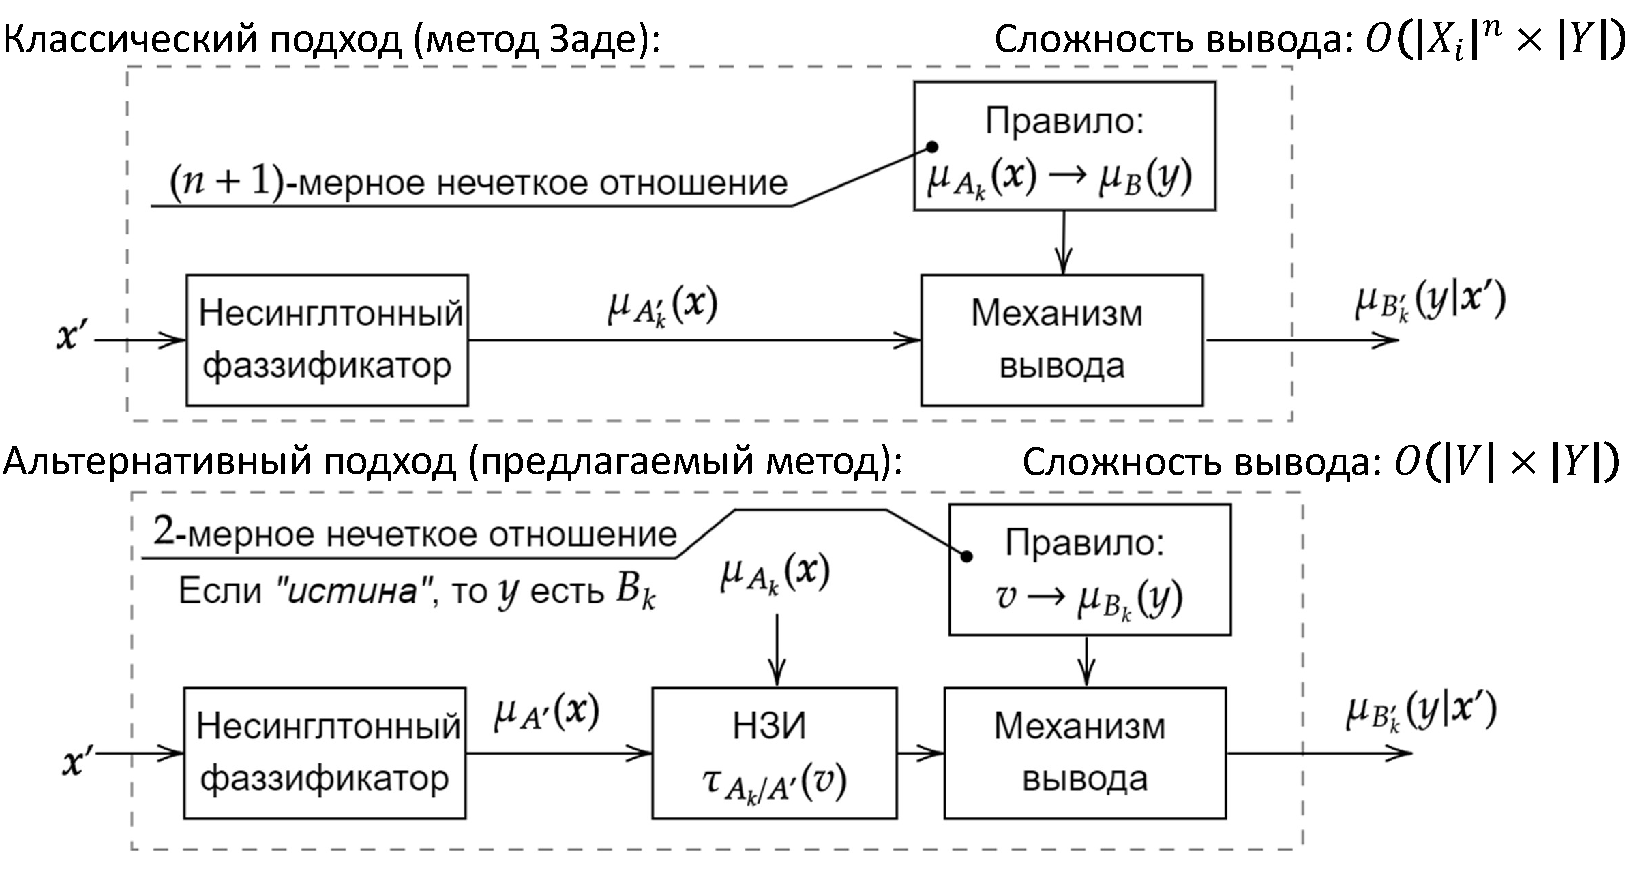
\includegraphics[scale=0.45]{ftv-schema-comparizon}
\caption{Сравнение классической схемы нечеткого вывода и схемы нечеткого вывода на основе НЗИ}
\label{fig:ftv-schema-comparizon}
\end{figure}

Порядок функции временной сложности вычисления $B'_k$ на основе выражения (\ref{eqn:ftv-compute-9}) составляет $O\left(n|V|^2+|V|\cdot |Y|\right)$, где $V=CP(A_k, A')$. Сравнение схем нечетких выводов с соответствии с соотношениями (\ref{eqn:fuz-problem-4}) и (\ref{eqn:ftv-compute-9}) представлены на рис. \cref{fig:ftv-schema-comparizon}.

\begin{figure}[th]
	\centering
	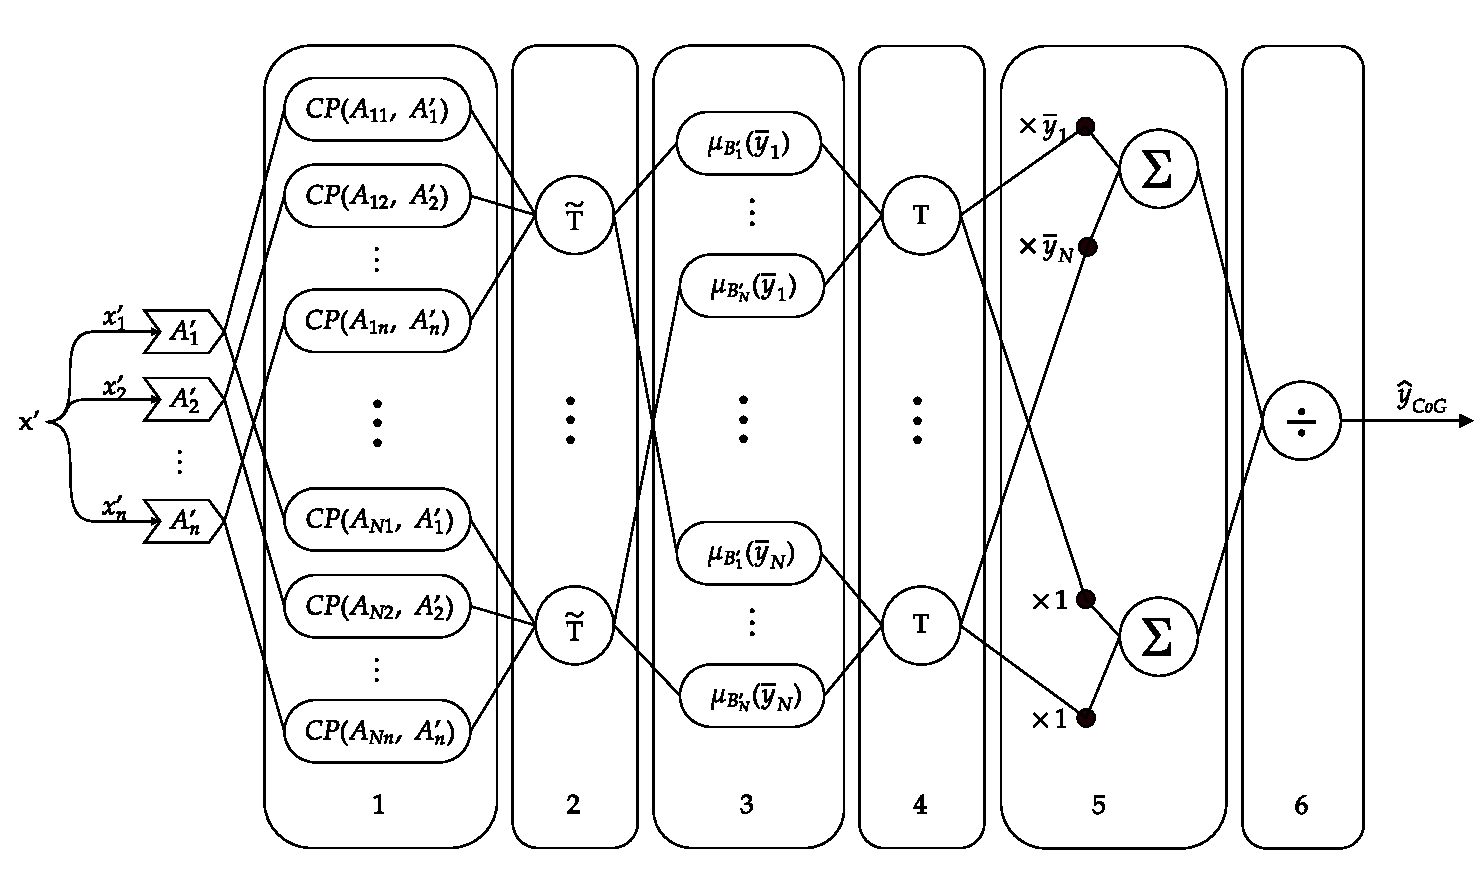
\includegraphics[scale=0.5]{neurofuzzysystem-defuzzification-cog}
	\caption{Схема нейро-нечеткой системы с использованием дефаззификации по методу центра тяжести}
	\label{fig:neurofuzzysystem-defuzzification-cog}
\end{figure}

Нейро-сетевая структура изображена на рисунке 

\begin{figure}[ht]
	\centering
	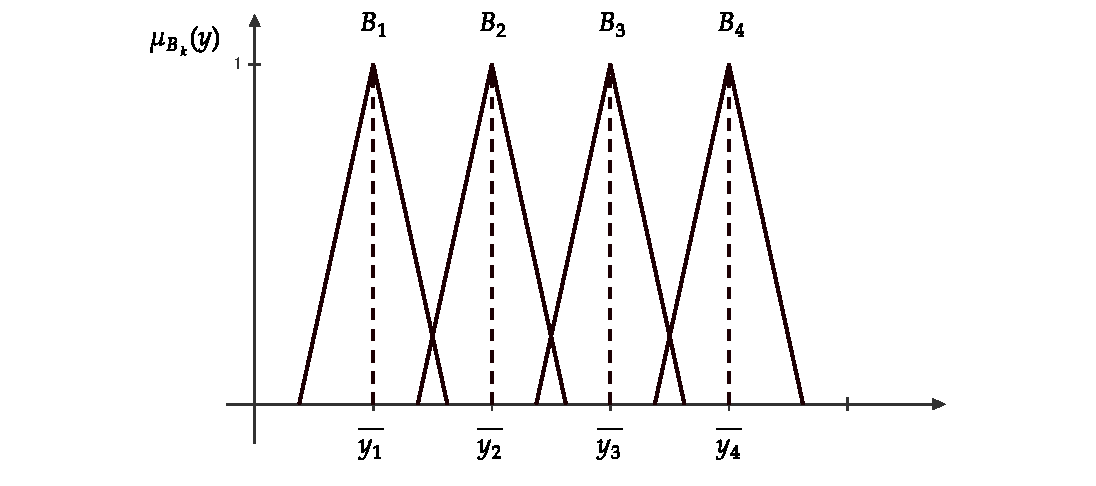
\includegraphics[scale=0.5]{out-mf-with-low-crossing}
	\caption{Пример нечетких множеств, удовлетворяющих условию $\mu_{B_k}(y_r) = 0$ для $y \ne r$.}
	\label{fig:out-mf-with-low-crossing}
\end{figure}

В \cite{Sinuk2023} ослаблено ограничение на использование одной и той же $T$-нормы в работах Менделя на примере вывода типа Мамдани, а также показано, что вывод по отдельному правилу при $T_2 = T_4 = T$ может быть записан через \textit{меру возможности}:
\begin{align*}
	\mu_{B'_k}(y) = \sup_{v\in[0;1]}\left\{\tau_{A_{k}|A'} \overset{\mathrm{T_2}}{\star} (v \overset{\mathrm{T_4}}{\star} \mu_{B_k}(y)) \right\} = \textstyle\prod_{\mathbf{A_k}|\mathbf{A'}} \overset{\mathrm{T}}{\star} \mu_{B_k}(y),
\end{align*}
где $\prod_{\mathbf{A_k}|\mathbf{A'}}=\sup_{v\in[0;1]}\left\{\tau_{A_{k}|A'} \overset{\mathrm{T}}{\star} v\right\}$.
Также в этой статье показана зависимость результата дефаззификации от ширины гауссовой функции принадлежности при использовании $T$-нормы Ларсена и дефаззификации \textit{по центру суммы}, в отличии от дефаззификации \textit{по среднему центру}.

Для предложенного метода вывода на основе нечеткого значения истинности в \cite{Karatach2024} показано, что для достаточно удаленных и непересекающихся выходных ф. п. нечетких множеств, т. е. когда $\mu_{B_k}(\bar{y}_r) = 0$ для $k \ne r$ (как изображено на рисунке \cref{fig:out-mf-with-low-crossing}), \todo{сложность вычисления дефаззификации по центру тяжести сокращается за счет упрощения выражений импликаций}.

Тогда для модели классификации

Тогда для модели регрессии.

\textbf{Третья глава} посвящена выработке эффективной параллельной реализации разработанного метода нечеткого вывода на основе нечеткого значения истинности с использованием технологии CUDA. В главе описан ключевые особенности организации вычисления нечеткого вывода при использовании технологии CUDA, параллельный алгоритм свертки НЗИ, особенности реализации методов дефаззификации в нечеткой модели регрессии и схема ускоренного вывода регрессионной нечеткой системы за счет предварительного отбора правил с ближайшими антецедентами.

{\color{red} ДОПИШУ:

Составлена конфигурация 

При дискретизированном вычисление ф. п. свертки НЗИ в некоторой точке расчетной сетки $v_j\in [0,1]$ потребуется просматривать значения НЗИ в отрезке $[v_j, 1]$, то есть имеет вычислительную сложность $O(D_{ftv})$, где $D_{ftv}$ --- число точек расчетной сетки ф. п. НЗИ. Таким образом вычисление свертки НЗИ по формуле (\ref{eqn:ftv-compute-11}) может быть распараллелено по точкам расчетной сетки, а нахождение $\tau_{\mathbf{A_k}|\mathbf{A'}}(v_j)$ использует операцию свертки, которая в имеет ограниченную возможность распараллеливания, но в целом требует большого количества повторных вычислений значений $\tau_{A_{ki}|A'_i}(v_k), v_k\in [v_j, 1]$. В \ref{alg:ftv-reduction} \cite{Karatach2024} предложен алгоритм вычисления свертки НЗИ сразу по всем входам с использованием техники динамического программирования, имеющий линейную зависимость от размера расчетной сетки $D_{ftv}$. Алгоритм приведен на \cref{alg:ftv-reduction}.
}

\begin{algorithm}
	\begin{algorithmic}
		\Require $ftv_i,\ i=\overline{1,n}$
		\State $max\_ftv[i] = 0;$
		\For{$v_j = 1\dots0$}
		\State $s \gets \left\{ftv_i[v_j] \mid ftv_i[v_j] >= max\_ftv[i]\right\};$
		\State $max\_ftv[i] \gets max(max\_ftv[i], ftv_i[v_j]);$
		\State $v\_max\_index \gets \mathrm{arg\,max}_i\left\{ftv_i[v_j]\right\};$
		\If{$s = \emptyset \And i = v\_max\_index$}
		\State $r[i] \gets ftv_{i}[v_j];$
		\Else
		\State $r[i] \gets max\_ftv[i];$
		\EndIf
		\State $ftv'[v_j] \gets \underset{i}{T_3}\left\{r[i]\right\}$;
		\EndFor
		\State \Return $ftv'$
	\end{algorithmic}
	\caption{Алгоритм свертки НЗИ при $T_1=min$ и $T_3(a, b) \ge T_3(c, d)$ если $a > c$ или $b > d$}
	\label{alg:ftv-reduction}
\end{algorithm}

\begin{figure}[ht]
	\centering
	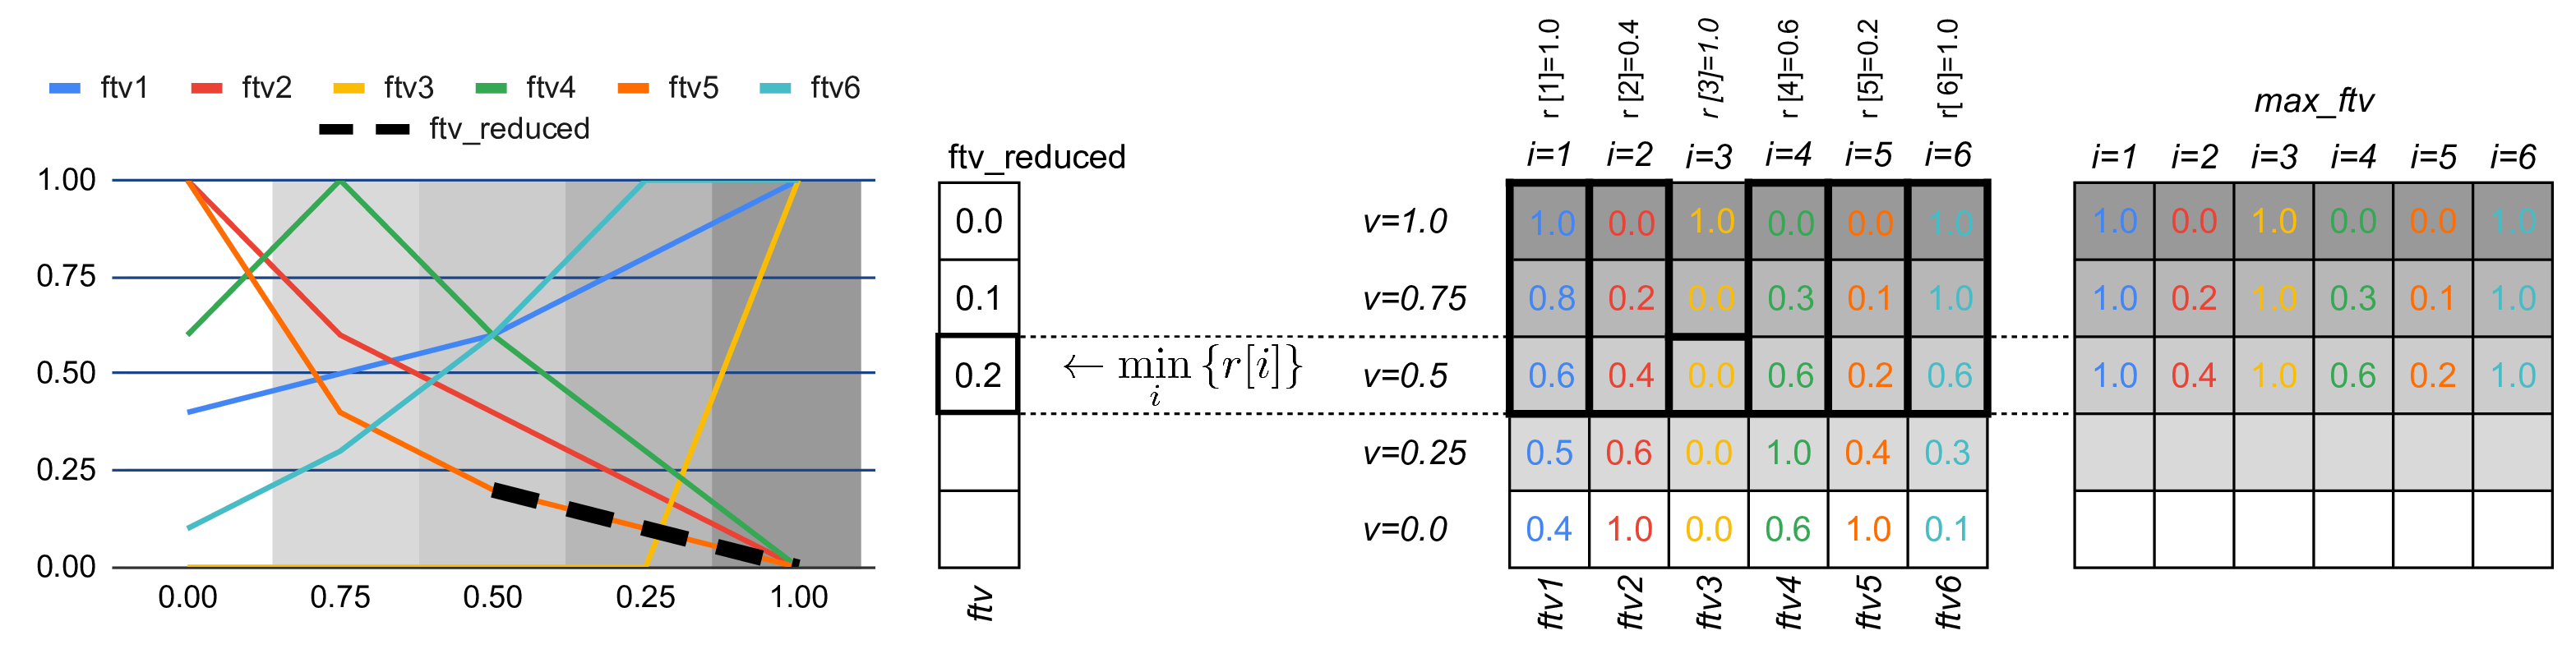
\includegraphics[width=\textwidth]{ftvs-reduction-example-gradient}
	\caption{Пример работы параллельного алгоритма свертки НЗИ при расчетной сетке состоящей из 5 точек.}
	\label{fig:ftvs-reduction-example}
\end{figure}

Для точного вычисления значения дефаззификации выхода нечеткой системы используется метод оптимизации \textit{Gradient-aware Particle Swarm Optimization}.



\textbf{Четвёртая глава} содержит описание нескольких проведенных экспериментов для оценки характеристик разработанной нечеткой модели прогнозирования временных рядов. Первый эксперимент направлен на подтверждение полиномиальной зависимости времени нечеткого вывода от количества входов нечеткой системы, а также на прирост качества прогнозирования при использовании нечеткого вывода логического типа с несинглтонной фаззификацией. Второй эксперимент был проведен для оценки качества в прикладной задаче прогнозирования временных рядов.

Первый эксперимент проводился с использованием синтетического набора данных Mackey-Glass (M-G). В данной работе этот набора данных был сгенерирован в результате решения дифференциального уравнения:
\begin{equation}
	\frac{dx(t)}{dt} = \beta\frac{x(t-\tau)}{1+x(t-\tau)^n}-\gamma x(t)
	\label{eqn:mackey-glass-definition},
\end{equation}
со значениями параметров $\tau = 30, \beta = 0.2, \gamma = 0.1$.

В эксперименте использовался участок временного ряда $t=\overline{1,1000}$, а также применялся адаптивный метод оценки зашумленности временной последовательности в каждой точке $t$ на основе экспоненциально взвешенного скользящего среднего.

\begin{figure}[ht]
	\begin{minipage}[c]{0.49\textwidth}
		\centering
		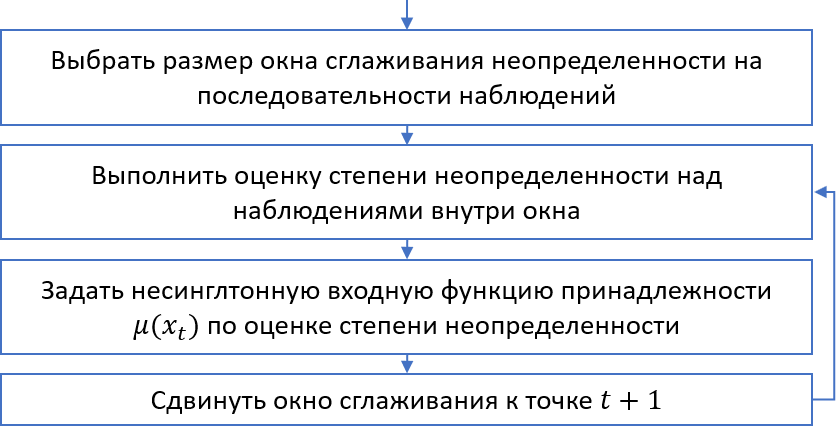
\includegraphics[width=\textwidth]{ns-procedure}
		\caption{Схема обобщенной процедуры адаптивной несинглтонной фаззификации временной последовательности.}
		\label{fig:ns-procedure}
	\end{minipage}
	\hfill
	\begin{minipage}[c]{0.49\textwidth}
		\centering
%		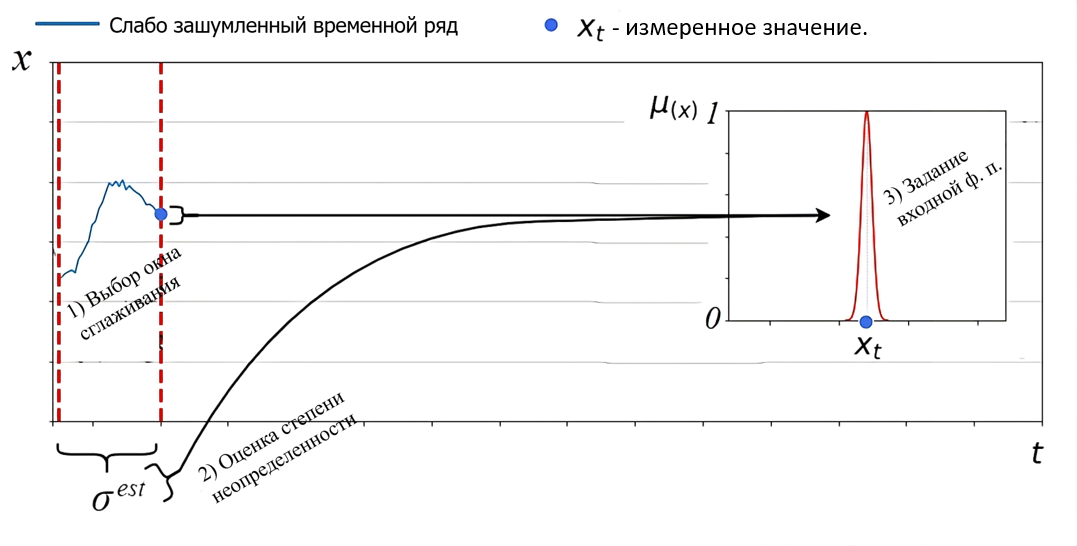
\includegraphics[width=\textwidth]{ns-demo-low-noise}
%		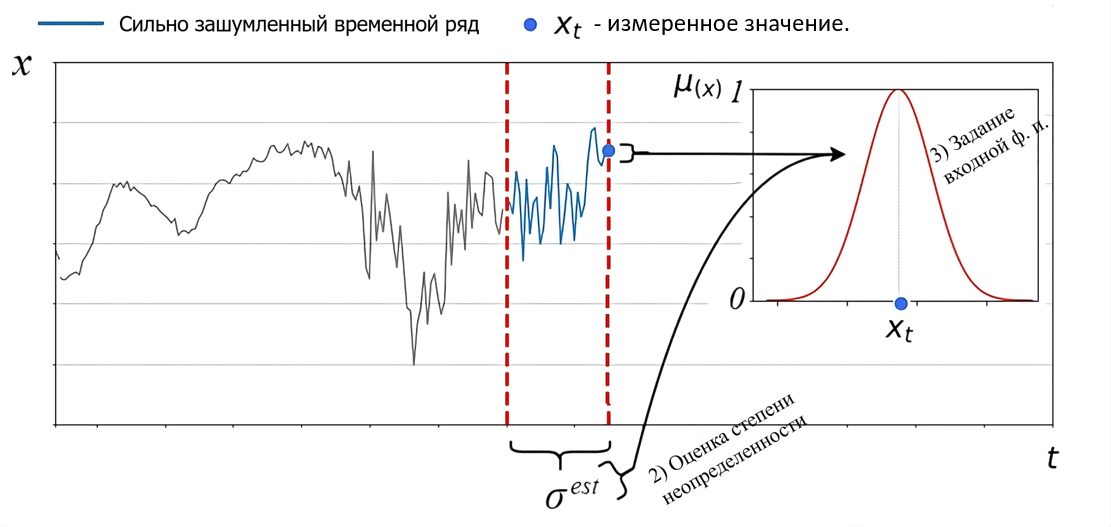
\includegraphics[width=\textwidth]{ns-demo-large-noise}
		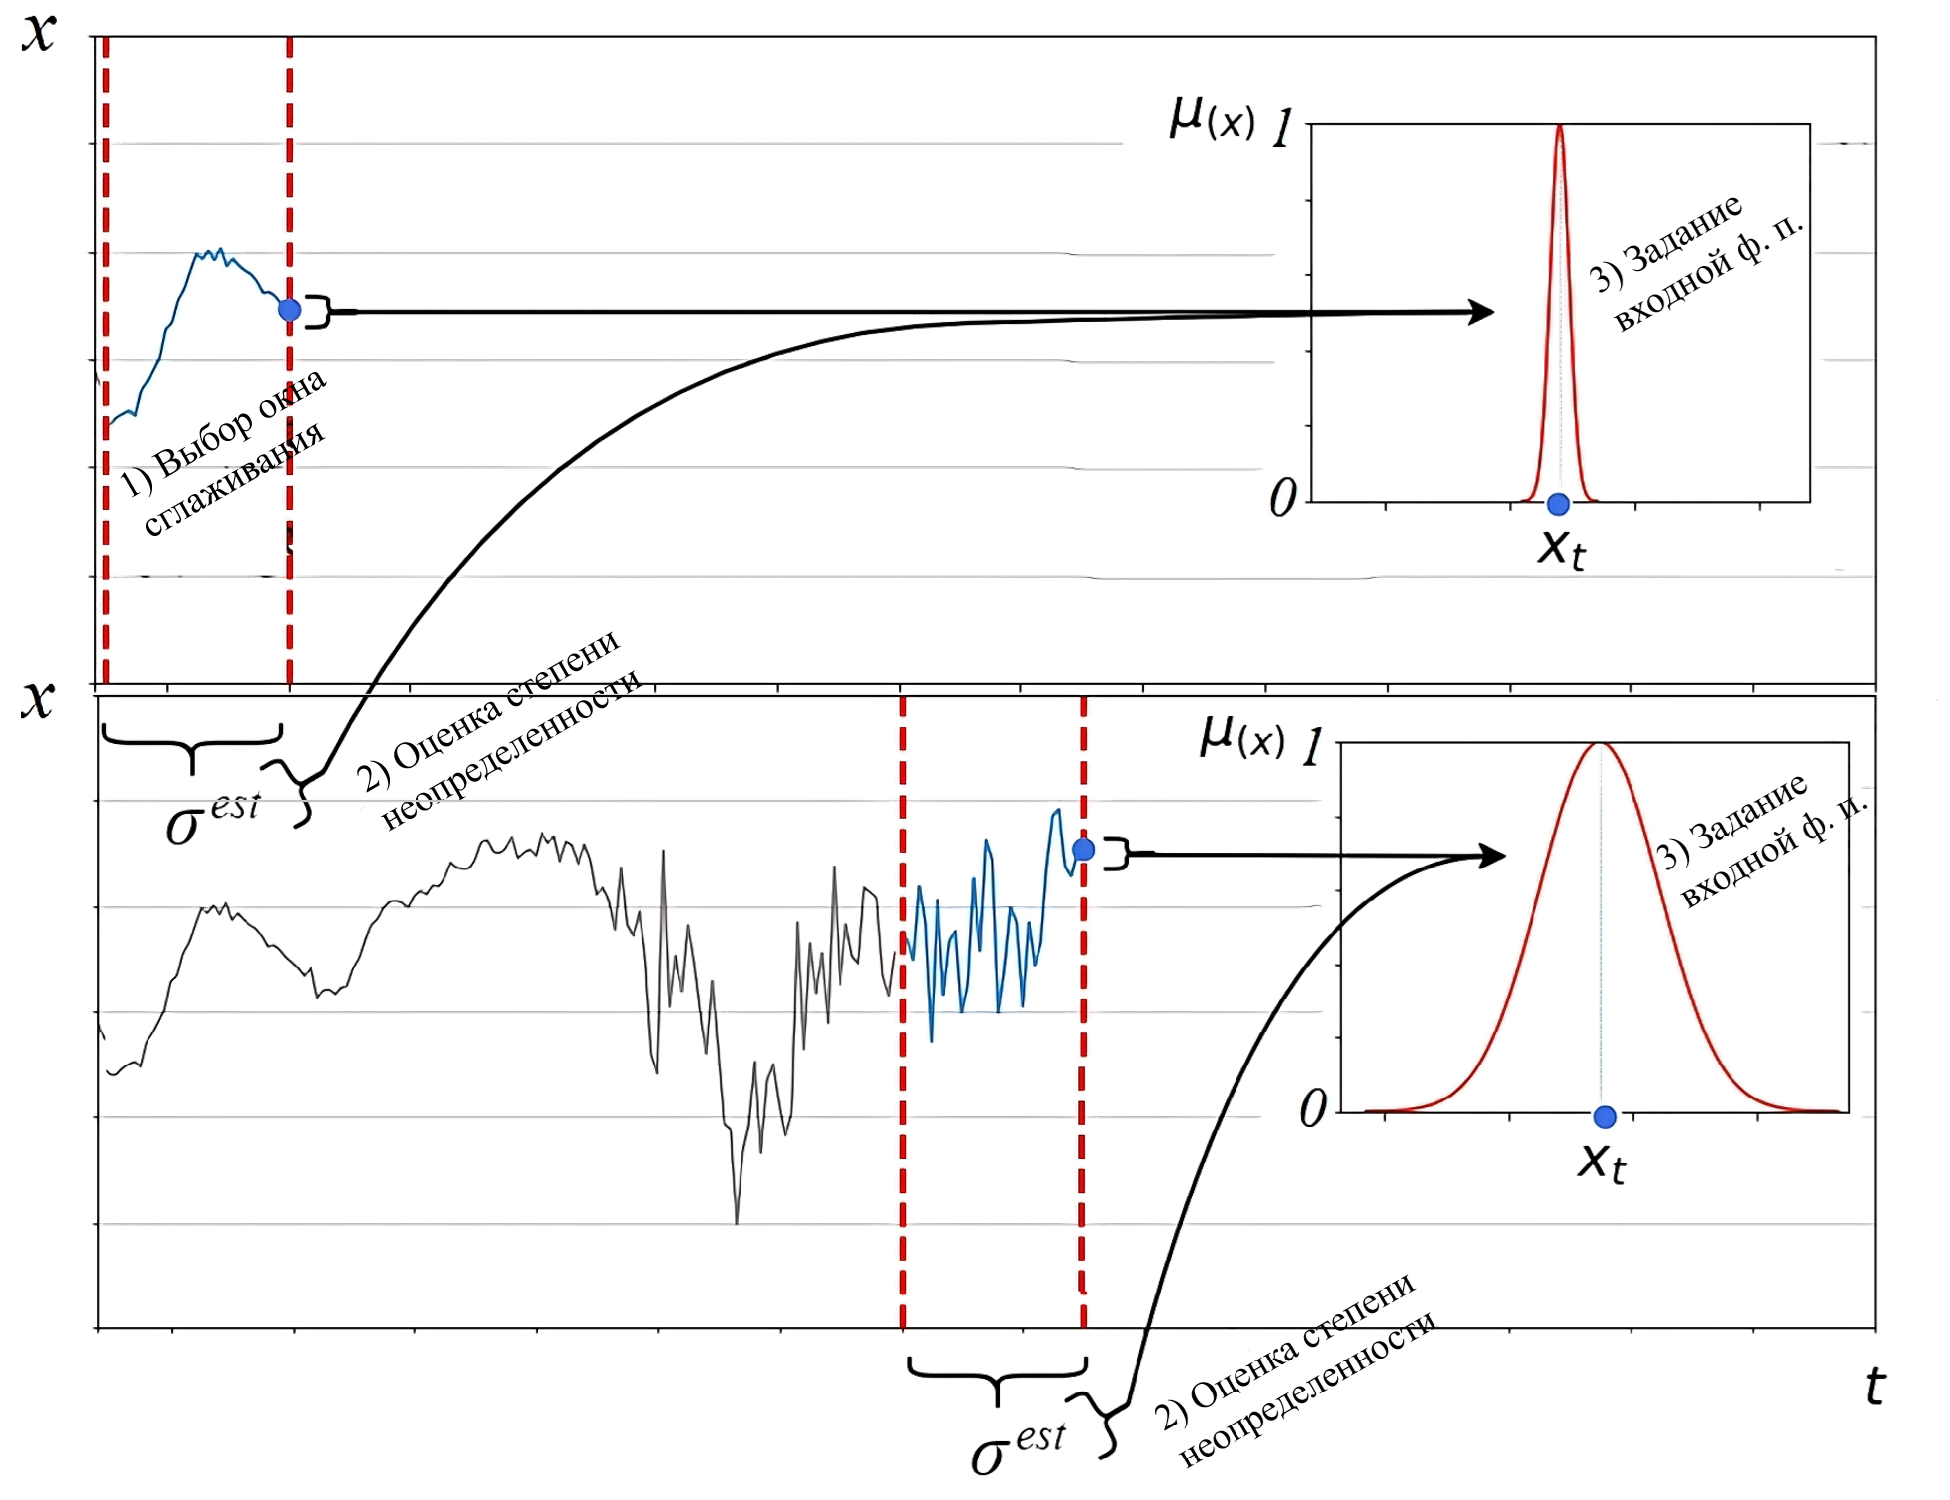
\includegraphics[width=\textwidth]{ns-demo-low-and-high-noise}
		\caption{Иллюстрация процедуры несинглтонной фаззификации временного ряда с низким (вверху) и высоким (внизу) уровнем шума.}
		\label{fig:ns-demo-low-and-high-noise}
	\end{minipage}
\end{figure}

Нечеткие множества для значений временного ряда были получены с использованием этой процедуры фаззификации временных рядов (\cref{fig:ns-procedure}) для обеспечения адаптивности оценки неопределенности в конкретной точке. Формулы для вычисления степени неопределенности показаны ниже%

\begin{minipage}{0.45\linewidth}
\begin{align}
	\label{eqn:mackey-glass-seq-diff}
	d_1 &= d_2, \notag \\
	d_t &= \frac{1}{\sqrt{2}}(x_t - x_{t-1}),
\end{align}
\begin{align}
	\hat{d}_t &= (1-\alpha) \hat{d}_{t-1} + \alpha d_t \notag \\
	&= \sum_{p=1}^t \alpha (1-\alpha)^{t-p} d_p. %\notag
	\label{eqn:mackey-glass-seq-diff-mean}
\end{align}
\end{minipage}\hfill
\begin{minipage}{0.45\linewidth}
\begin{align}
	\hat{\sigma}^2_t &= (1-\alpha) \hat{\sigma}^2_{t-1} + \alpha (d_t - \hat{d}_t) \notag \\
	&= \sum_{p=1}^t \alpha (1-\alpha)^{t-p} (d_p - \hat{d}_p)^2, \label{eqn:mackey-glass-seq-diff-var-iterative} \\
	\hat{\sigma}_t &= \sqrt{\hat{\sigma}^2_t}, \label{eqn:mackey-glass-seq-diff-std}
\end{align}
\end{minipage}

\begin{figure}[ht]
	\centering
	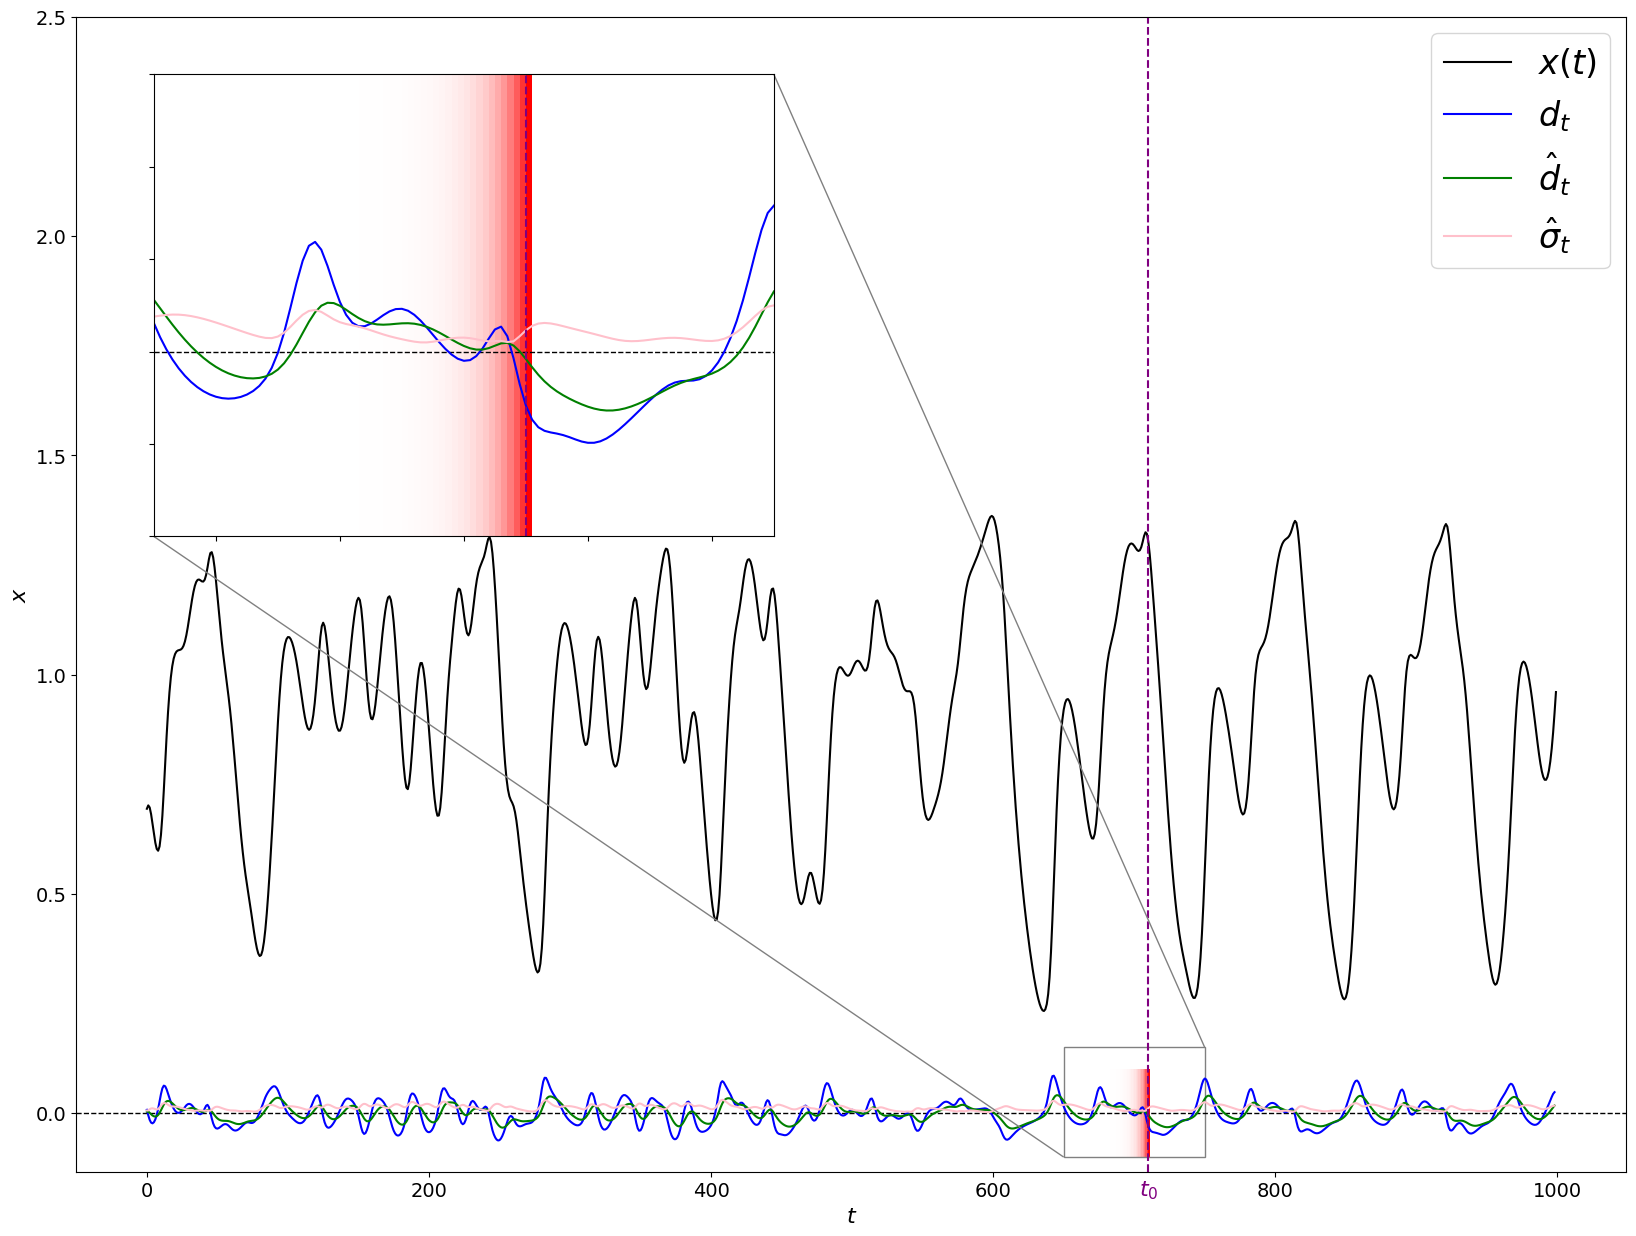
\includegraphics[scale=0.3]{mackey-glass-ewma-example}
	\caption{График сгенерированной последовательности Mackey-Glass $x(t), t\in[0;999]$, график разностей соседних точек $d_t$ последовательности $x(t)$, график $\hat{d}_t$ с наложением экспоненциально взвешенного сглаживания на последовательность разностей и график экспоненциально взвешенного скользящего среднеквадратичного отклонения разностей $\hat{\sigma}_t$. На вложенном изображении участка $t\in[650,750]$ яркостью красного цвета показано значения весового коэффициента $\alpha (1-\alpha)^{t-p}, p=\overline{1,t_0}$ при $\alpha = 0.2$.}
	\label{fig:mackey-glass-ewma-example}
\end{figure}

\begin{figure}[tbh]
	\centering
	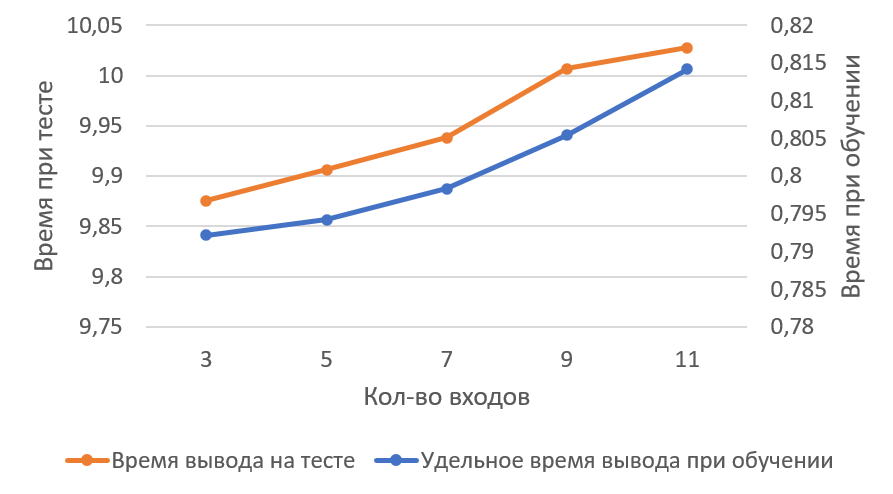
\includegraphics[scale=0.7]{mackey-glass-inference-duration}
	\caption{График длительности выполнения параллельной реализации нечеткого вывода для обучающего и тестового набора данных при количестве правил $N=30$.}
	\label{fig:mackey-glass-inference-duration}
\end{figure}

После проведенного вычислительного эксперимента были получены показатели удельного (на одну точку из набора точек одной итерации алгоритма PSO) времени работы параллельного алгоритма нечеткого вывода на основе НЗИ на обучающем наборе данных и времени работы на тренировочном наборе данных для различного размера окна запаздывания, изображенные на рисунке \cref{fig:mackey-glass-inference-duration}. На этом рисунке наблюдается линейный рост времени выполнения алгоритма с увеличением количества входов нечеткой системы, что \textbf{подтверждает утверждение о полиномиальной зависимости временной сложности метода нечеткого вывода на основе НЗИ от количества входов}.

Для сравнения с альтернативными нечеткими моделями условия этого эксперимента были выбраны такими же как в публикации \cite{}, приводящей результаты прогнозирования временного ряда M-G для нечетких систем типа Мамдани при синглтонной и несинглтонной фаззификации. Качество прогнозирования оценивалось с использованием метрики sMAPE:
\[
sMAPE = \frac{100\%}{n} \sum_{t=1}^n 
\frac{|y_t - \hat{y}_t|}{\tfrac{|y_t| + |\hat{y}_t|}{2}},
\]
где $y_t$ и $\hat{y}_t$ соответствуют истинному и предсказанному значению в момент времени $t$.

\begin{figure}
	\centering
	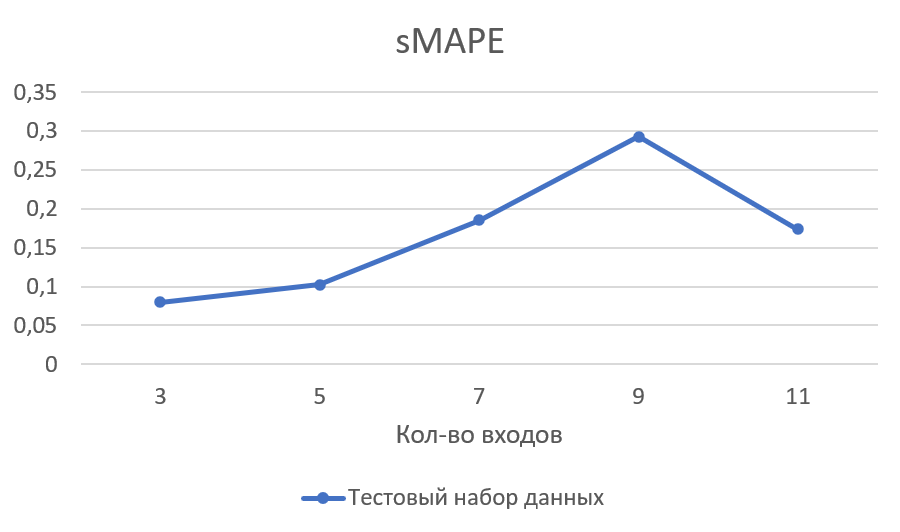
\includegraphics[scale=0.7]{mackey-glass-inference-smape}
	\caption{График значений метрики sMAPE на обучающем и тестовом наборах данных при различных размерах окна запаздывания, количестве правил --- 30.}
	\label{fig:mackey-glass-inference-smape}
\end{figure}

По итогу проведенного эксперимента лучший показатель качества прогнозирования по этой метрике на рисунке \cref{fig:mackey-glass-inference-smape} достигается при размере окна запаздывания --- 3 точки. 

Достигнутое в этом случае значение $sMAPE = 8\%$ при количестве правил 30, заметно превосходит точность моделирования незашумленной последовательности Mackey-Glass (M-G) с использованием синглтонной фаззификации со значением $sMAPE \approx 40\%$ в \cite{Pekaslan2020}. Также полученное качество прогнозирования сопоставимо со значением этой метрики при аналогичной конфигурации эксперимента прогнозирования временного ряда M-G в той же публикации, где для достижения точности моделирования временной последовательности $sMAPE \approx 10\%$ используется нечеткая система типа Мамдани, содержащая 184 правила\footnote{Непосредственно в самой статье не указано количество используемых правил. Однако авторами этой статьи опубликован программный код описанного в статье метода, запустив который удалось воспроизвести проводимые авторами эксперименты и восстановить количество правил в их нечетких системах.} в базе правил для не зашумленного временного ряда M-G и 597, 402, 312 правил для различных конфигураций и амплитуды добавленного шума. Данные наблюдения показывают, что \textbf{метод регрессии временных рядов на основе логического нечеткого вывода при несинглтонной фаззификации значительно превосходит качество регрессии с использованием синглтонной фаззификации, а также имеет сопоставимую с методом регрессии Мамдани при несинглтонной фаззификации точность, но при меньшем количестве правил} за счет возможности построения более сложной функции аппроксимации.

Второй эксперимент посвящен применению разработанного метода для прогнозирования помесячного объема транзакций безналичных платежей корпоративным клиентам банка. Источником неопределенности в этом наборе данных является стохастический характер динамики временной последовательности. Поэтому в этом эксперименте также использовалась процедура адаптивной несинглтонной фаззификации. В качестве метрики использовалась RMAE (relative MAE) --- отношение средней абсолютной ошибки к математическому ожиданию средних по рядам клиентов:
\[
RMAE = \frac{MAE}{\mathbb{E}[\mathbb{E}[s_t]]}.
\]

По итогу эксперимента было получено значение метрики $RMAE = 0.112/0.147$ при прогнозировании на один/три месяца соответственно. Это превосходит на $12\%/5\%$ качество прогнозирования с использованием многослойного перцептрона со значениями $RMAE = 0.128/0.157$. 




%В заключении перечислены основные научные результаты, каждый из которых подтверждён приведёнными формулами, схемами, экспериментальными графиками и таблицами: (1) формализация и аналитическая реализация метода на основе НЗИ; (2) снижение вычислительной сложности и эффективная параллельная реализация; (3) экспериментальная оценка на реальных задачах; (4) создание программной системы с поддержкой GPU и интеграцией в Python.

В \textbf{заключении} сделаны выводы о полученных в процессе работы результаты.

\pdfbookmark{Заключение}{conclusion}                                  % Закладка pdf
\section*{Заключение}
В результате выполнения работы удалось выработать метод нечеткого вывода на основе нечеткого значения истинности, позволяющий использовать тип фаззификации non-singleton при полиномиальной сложности вывода от количества входов, а также показано улучшение качества прогнозирования временных рядов с использованием логического типа вывода в сравнении с синглтонной фаззификацией и выводом типа Мамдани. В работе решены поставленные задачи и получены следующие результаты:
%% Согласно ГОСТ Р 7.0.11-2011:
%% 5.3.3 В заключении диссертации излагают итоги выполненного исследования, рекомендации, перспективы дальнейшей разработки темы.
%% 9.2.3 В заключении автореферата диссертации излагают итоги данного исследования, рекомендации и перспективы дальнейшей разработки темы.
\begin{enumerate}
  \item Анализ состояния исследований в области анализа качественных/за­шумленных данных с использованием нечеткого моделирования показал недостатки существующих методов. В частности, было выявлено отсут­ствие таких методов для моделирования систем и процессов, имеющих множество качественных/зашумленных входов, которые работали бы с полиномиальной вычислительной сложностью от количества входов и не были бы связаны со значительными упрощениями теории нечеткого логического вывода.
  \item Для логического подходов были разработаны методы, позволяющие осуществлять нечеткий логиеский вывод с полиномиаль­
  ной сложностью для произвольного набора используемых t-норм, что обеспечивает более гибкую настройку таких систем. Для определенных частных случаев в наборах используемых норм были разработаны опти­мизированные версии этих методов с использованием меры возможности.
  \item Разработан метод классификации для объектов со многими нечеткими входах\ldots
  \item Математическое моделирование показало \ldots
  \item Для выполнения поставленных задач был создан \ldots
\end{enumerate}


\pdfbookmark{Литература}{bibliography}                                % Закладка pdf
%При использовании пакета \verb!biblatex! список публикаций автора по теме
%диссертации формируется в разделе <<\publications>>\ файла
%\verb!common/characteristic.tex!  при помощи команды \verb!\nocite!

\ifdefmacro{\microtypesetup}{\microtypesetup{protrusion=false}}{} % не рекомендуется применять пакет микротипографики к автоматически генерируемому списку литературы
\urlstyle{rm}                               % ссылки URL обычным шрифтом
\ifnumequal{\value{bibliosel}}{0}{% Встроенная реализация с загрузкой файла через движок bibtex8
	\renewcommand{\bibname}{\large \bibtitleauthor}
	\nocite{*}
	\insertbiblioauthor           % Подключаем Bib-базы
	%\insertbiblioexternal   % !!! bibtex не умеет работать с несколькими библиографиями !!!
}{% Реализация пакетом biblatex через движок biber
	% Цитирования.
	%  * Порядок перечисления определяет порядок в библиографии (только внутри подраздела, если `\insertbiblioauthorgrouped`).
	%  * Если не соблюдать порядок "как для \printbibliography", нумерация в `\insertbiblioauthor` будет кривой.
	%  * Если цитировать каждый источник отдельной командой --- найти некоторые ошибки будет проще.
	%
	%% authorvak
	\nocite{Karatach2023}%
	\nocite{Karatach2021}%
	\nocite{vakbib3}%
	\nocite{vakbib4}%
	\nocite{vakbib5}%
	\nocite{vakbib6}%
	\nocite{vakbib7}%
	\nocite{vakbib8}%
	\nocite{vakbib9}%
	\nocite{vakbib10}%
	\nocite{vakbib11}%
	\nocite{vakbib12}%
	%
	%% authorwos
	\nocite{Karatach2024}%
	\nocite{Sinuk2023}%
	\nocite{wosbib1}%
	%
	%% authorscopus
	\nocite{Karatach2023b}%
	%
	%% authorpatent
	\nocite{patbib1}%
	%
	%% authorconf
	\nocite{Karatach2020}%
	\nocite{Karatach2021parallel}%
	\nocite{Sinuk2022}%
	\nocite{Karatach2022}%
	\nocite{confbib2}%
	%
	%% authorother
	\nocite{bib1}%
	\nocite{bib2}%
	%
	%% authorprogram
	\nocite{Rospatent1}%
	\nocite{Rospatent2}%
	
	\ifnumgreater{\value{usefootcite}}{0}{
		\begin{refcontext}[labelprefix={}]
			\ifnum \value{bibgrouped}>0
			\insertbiblioauthorgrouped    % Вывод всех работ автора, сгруппированных по источникам
			\else
			\insertbiblioauthor      % Вывод всех работ автора
			\fi
		\end{refcontext}
	}{
		\ifnum \totvalue{citeexternal}>0
		\begin{refcontext}[labelprefix=A]
			\ifnum \value{bibgrouped}>0
			\insertbiblioauthorgrouped    % Вывод всех работ автора, сгруппированных по источникам
			\else
			\insertbiblioauthor      % Вывод всех работ автора
			\fi
		\end{refcontext}
		\else
		\ifnum \value{bibgrouped}>0
		\insertbiblioauthorgrouped    % Вывод всех работ автора, сгруппированных по источникам
		\else
		\insertbiblioauthor      % Вывод всех работ автора
		\fi
		\fi
		%  \insertbiblioauthorimportant  % Вывод наиболее значимых работ автора (определяется в файле characteristic во второй section)
		\begin{refcontext}[labelprefix={}]
			\insertbiblioexternal            % Вывод списка литературы, на которую ссылались в тексте автореферата
		\end{refcontext}
		% Невидимый библиографический список для подсчёта количества внешних публикаций
		% Используется, чтобы убрать приставку "А" у работ автора, если в автореферате нет
		% цитирований внешних источников.
		\printbibliography[heading=nobibheading, section=0, env=countexternal, keyword=biblioexternal, resetnumbers=true]%
	}
}
\ifdefmacro{\microtypesetup}{\microtypesetup{protrusion=true}}{}
\urlstyle{tt}                               % возвращаем установки шрифта ссылок URL















\newpage

\section{Постановка задачи нечеткого логического вывода}

Лингвистическая модель представляет собой базу правил вида:
\begin{equation}
	\label{eqn:fuz-problem-1}
	R_k:\ \text{Если}\ x_1\ \text{есть}\ A_{k1}\ \text{и}\ x_2\ \text{есть}\ A_{k2}\ \text{и} \dots \text{и}\ x_n\ \text{есть}\ A_{kn}, \text{то}\ y\ \text{есть}\ B_k,
\end{equation}
где $N$ "--- количество нечетких правил, $A_{ki} \subseteq X_i, i=\overline{1,n}, B_k \subseteq Y$"--- нечеткие множества, которые характеризуются функциями принадлежности $\mu_{A_{ki}}(x_i)$ и $\mu_{B_k}(y)$ соответственно; $x_1, x_2,…,x_n$"--- входные переменные лингвистической модели, причем
\[
[x_1, x_2, ..., x_n]^T = \mathbf{x} \in X_1 \times X_2 \times \dots \times X_n.
\]

Символами  $X_i, i=\overline{1,n}$ и $Y$ обозначаются соответственно пространства входных и выходной переменных. Если ввести обозначения $\mathbf{X}=X_1 \times X_2 \times \dots \times X_n$ и $\mathbf{A_k}=A_{k1}\times A_{k2} \times \dots \times A_{kn}$ , причем
\[
\mu_\mathbf{A_k}(\mathbf{x}) = \underset{i=\overline{1,n}}{T_1} \mu_{A_{ki}}(x_i),
\]
где $T_1$ - произвольная $t$-норма, то правило \ref{eqn:2.1} представляется в виде нечеткой импликации
\begin{equation}
	\label{eqn:fuz-problem-2}
	R_k: \mathbf{A_k} \to B_k, k=\overline{1,N}.
\end{equation}

Правило $R_k$ можно формализовать как нечеткое отношение, определенное на множестве  $\mathbf{X}\times Y$, т.е. $R_k \subseteq \mathbf{X} \times Y$ - нечеткое множество с функцией принадлежности
\[
\mu_{R_k}(\mathbf{x}, y) = \mu_{\mathbf{A_k} \to B_k} (\mathbf{x}, y).
\]

Модель логического типа определяет задание функции $\mu_{\mathbf{A_k} \to B_k} (\mathbf{x}, y)$ на основе известных функций принадлежности $\mu_{\mathbf{A_k}}(\mathbf{x})$ и $\mu_{B_k}(y)$ с помощью одной из предложенных в [2] функций импликации:
\[
\mu_{\mathbf{A_k} \to B_k} (\mathbf{x}, y) = I(\mu_{\mathbf{A_k}}(\mathbf{x}), \mu_{B_k}(y)),
\]
где $I$"--- некоторая импликация.

Ставится задача определить нечеткий вывод $B'_k \subseteq Y$ для системы, представленной в виде (\ref{eqn:2.1}), если на входах - нечеткие множества.
$\mathbf{A'}=A'_1 \times A'_2 \times \dots \times A'_n \subseteq \mathbf{X}$ или $x_1\ \text{есть}\ A'_1\ \text{и}\ x_2\ \text{есть}\ A'_2\ \text{и} \dots \text{и}\ x_n\ \text{есть}\ A'_n$  с соответствующей функцией принадлежности $\mu_{\mathbf{A'}}(\mathbf{x})$, которая определяется как
\begin{equation}
	\label{eqn:fuz-problem-3}
	\mu_{\mathbf{A'}}(\mathbf{x}) = \underset{i=\overline{1,n}}{T_3} \mu_{A'_i}(x_i).
\end{equation}

Несинглтонный фаззификатор отображает измеренное $x_i=x'_i, i=\overline{1,n}$ в нечеткое число, для которого $\mu_{A'_i}(x'_i) = 1$ и $\mu_{A'_i}(x_i)$ уменьшается от единицы по мере удаления от  $x'_i$.
В соответствии с обобщенным нечетким правилом modus ponens [2], нечеткое множество $B'_k$ определяется композицией нечеткого множества $\mathbf{A'}$ и отношения $\mathbf{R_k}$, т.е.
\[
B'_k = \mathbf{A'} \circ (\mathbf{A_k} \to B_k),
\]
или, на уровне функций принадлежности
\begin{equation}
	\label{eqn:fuz-problem-4}
	\mu_{B'_k}(y|\mathbf{x'}) = \sup_{\mathbf{x}\in \mathbf{X}}\left\{\mu_{\mathbf{A'}}(\mathbf{x'})\overset{T_2}{\star} I(\mu_{\mathbf{A_k}}(\mathbf{x}), \mu_{B_k}(y))\right\}.
\end{equation}

В (\ref{eqn:fuz-problem-4}) применена условная нотация, так как ввод в нечеткую систему происходит при определенном значении $\mathbf{x}$, а именно $\mathbf{x'}$. Обозначение $\mu_{B'_k}(y | \mathbf{x'})$ показывает, что $\mu_{B'_k}$ изменяется с каждым значением $\mathbf{x'}$. \textbf{Вычислительная сложность выражения (\ref{eqn:fuz-problem-4}) составляет $O(|X_1|\cdot |X_2|\cdot \dots \cdot |X_n|\cdot |Y|)$ т.е. экспоненциальная.}

\section{Использование нечетких систем для прогнозировани временных рядов}

В основной доле публикаций, касающихся использования фаззификации типа non-singleton, рассматривается задача прогнозирования временных рядов. В этих работах используются нечеткие системы типа Мамдани и Такаги-Сугено, тогда как в публикации \cite{} было показано увеличение точности моделирования при использовании нечеткой логической системы с импликацией Лукасевича. Также, согласно , нечеткая логическая система позволяет строить более сложную функцию аппроксимации при меньшем количестве правил. 

Процедура решения задачи прогнозирования временного ряда с использованием нечеткой логической модели состоит из следующих шагов:
\begin{enumerate}
	\item Выявление источника неопределенности значений временной последовательности. Источниками неопределенности для временного ряда могут выступать: ошибки измерений (шум, округление), потеря информации при агрегации собранных данных, а также стохастическая природа процесса генерации данных или структурные сдвиги.
	\item Для выявленного источника неопределенности следует выразить математически способ числовой оценки степени неопределенности, на основе которой можно определить форму и положение функции принадлежности в процедуре фаззификации.
	\item Выбирается целевая метрика, наиболее корректно оценивающая качество прогнозирования временного ряда в рамках задачи.
	\item Набор данных временных рядов разбивается на обучающий и тестовый диапазоны.
	\item Далее в качестве модели прогнозирования временного ряда используется нечеткая логическая система. Часть параметров модели фиксируются интуитивно экспертом исследователем, часть подбирается перебором или, например, с использованием Байесовской оптимизации, а оставшиеся параметры подбираются алгоритмом оптимизации. Для алгоритма оптимизации выбирается оптимизируемая функция, которая может отличаться от целевой метрики.
	\item Для полученного набора правил проводится оценка качества моделирования на отложенном тестовом диапазоне данных по целевой метрике.
\end{enumerate}


\subsection{Процедура несинглтонной фаззификации временных последовательностей}

\begin{figure}[tb!]
	\centering
	\begin{minipage}[b]{0.48\textwidth}
		\centering
		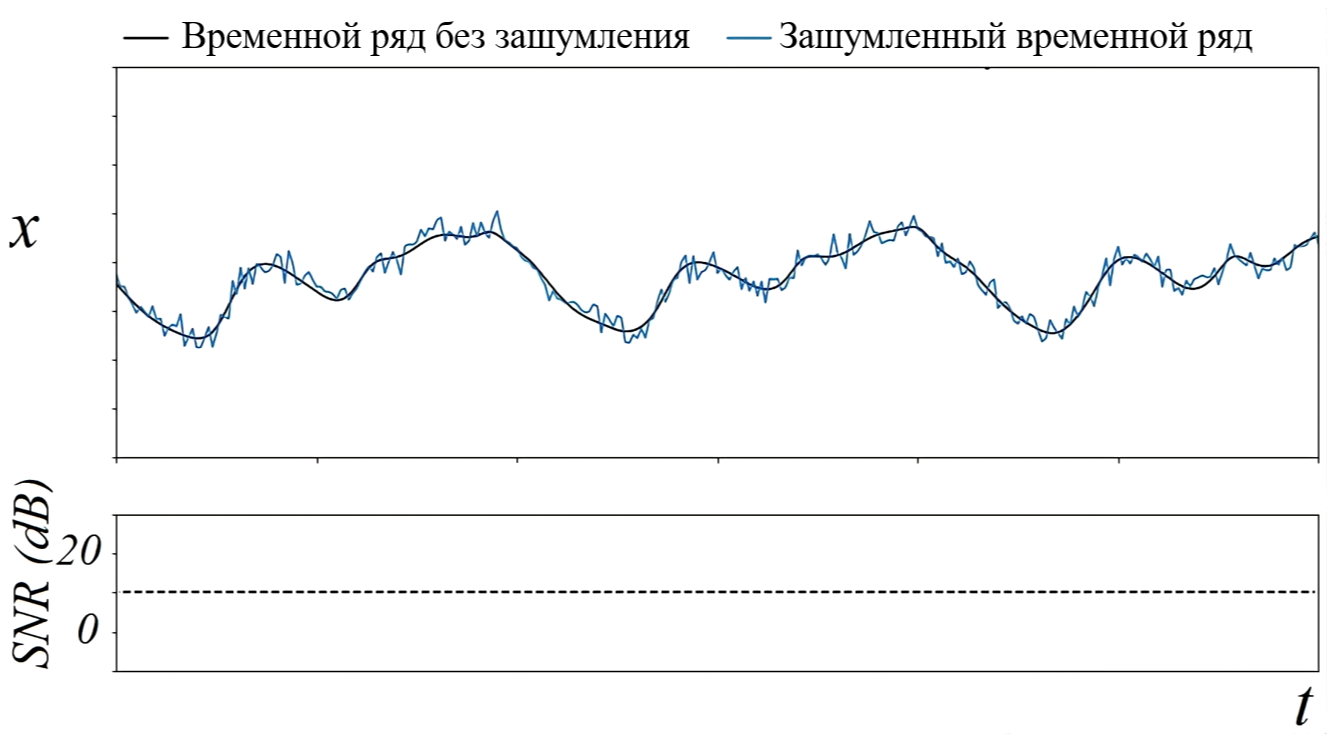
\includegraphics[width=\textwidth]{noisy-ts-demo-stable-noise}
		\caption*{а}
	\end{minipage}
	\hfill
	\begin{minipage}[b]{0.48\textwidth}
		\centering
		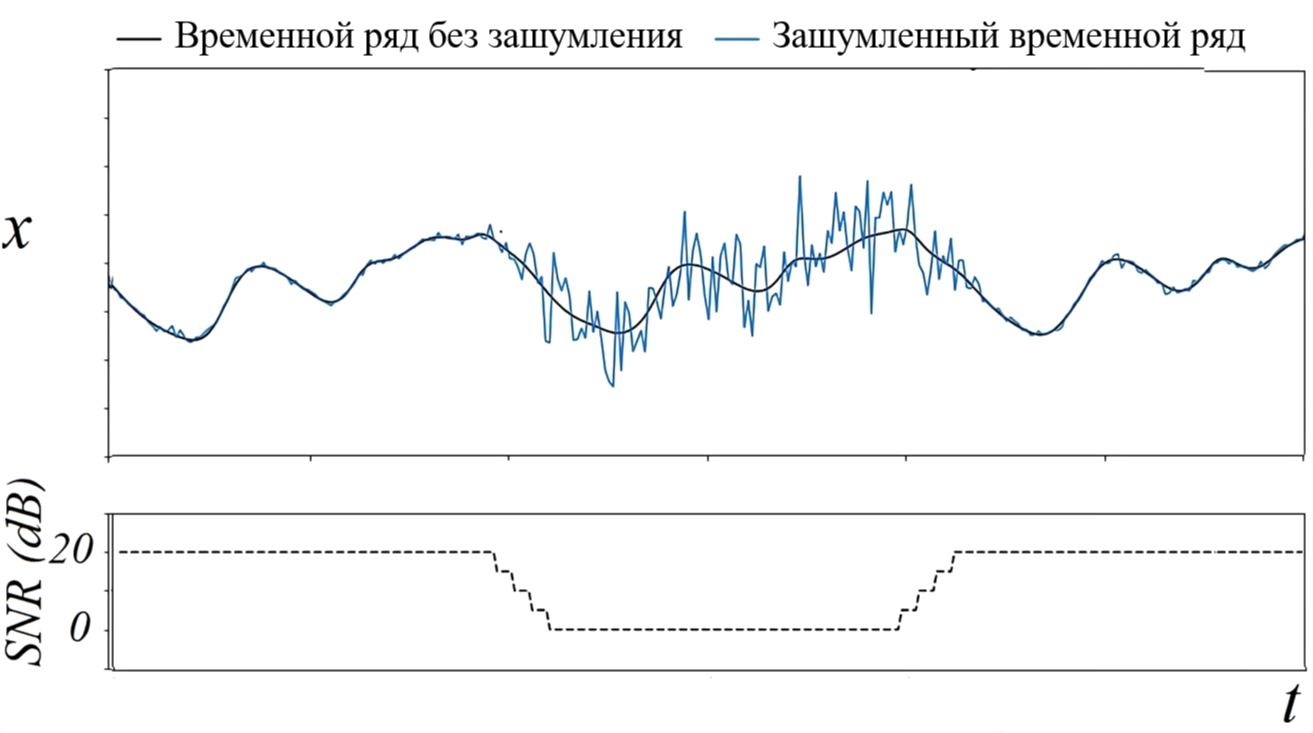
\includegraphics[width=\textwidth]{noisy-ts-demo-mixed-stable-noise}
		\caption*{б}
	\end{minipage}
	\vspace{0.5em}
	
	\begin{minipage}[b]{0.48\textwidth}
		\centering
		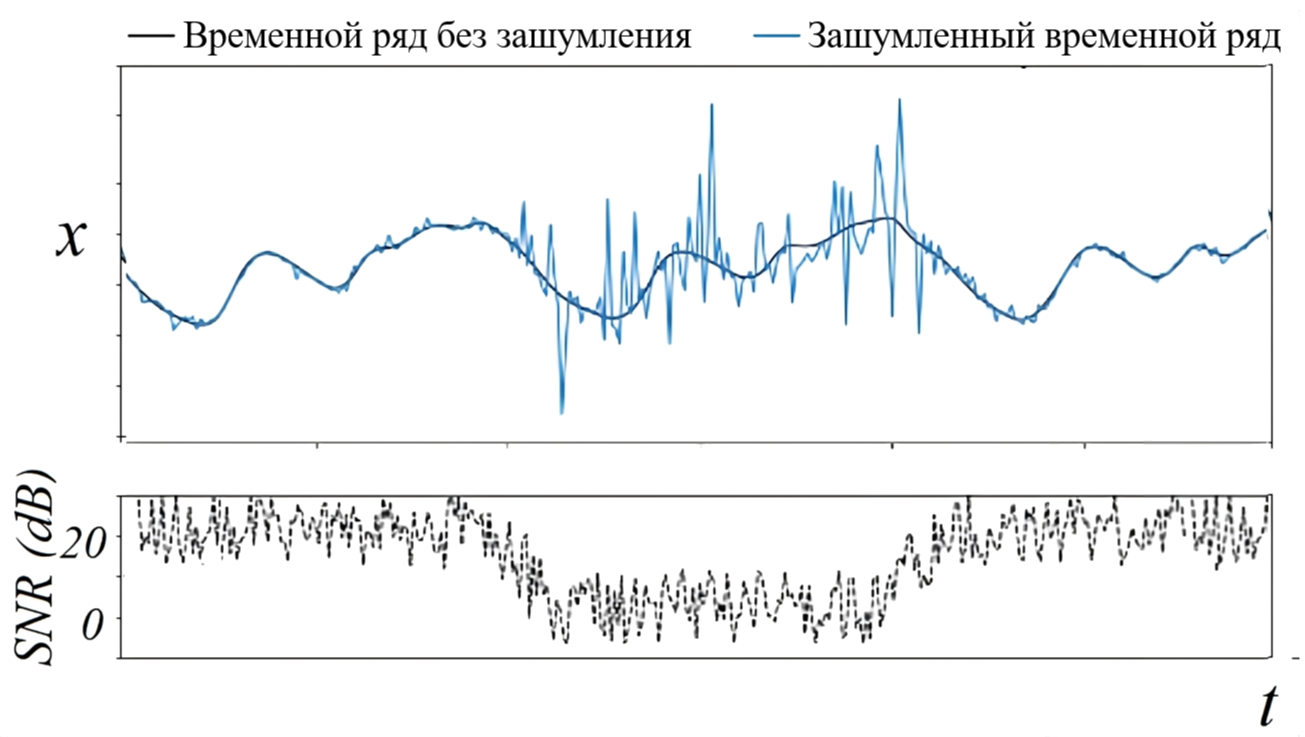
\includegraphics[width=\textwidth]{noisy-ts-demo-variable-noise}
		\caption*{в}
	\end{minipage}
	\caption{Примеры временных рядов с различными типами шума: (а) стабильный шум, (б) смешанный стабильный шум, (в) переменный шум. $SNR(dB) = 10 \log_{10} \frac{\sigma^2_s}{\sigma^2_n}$ --- отношение среднеквадратичного значения сигнала $\sigma^2_s$ к среднеквадратичному значению шума $\sigma^2_n$ (ОСШ, \textit{signal-to-noise ratio}) в децибелах. Большее значение $SNR(dB)$ соответствует меньшему уровню шума.}
	\label{fig:noisy-ts-demo}
\end{figure}

В задаче прогнозирования временных рядов измеренные значения могут содержать в себе неопределенность, зачастую возникающую из-за шумового искажения измерений. Такая неопределенность может выражена при сопоставлении каждому измеренному значению несинглтонной функции принадлежности нечеткого множества. \textbf{\textit{Концептуально предполагается, что поступающие на вход данные $x$ --- это значение, которое, вероятно, является правильным, но из-за существующей неопределенности соседние значения $x$ также потенциально могут быть правильными. По мере удаления от входного значения $x$ вероятность того, что оно будет правильным уменьшается. Таким образом, несинглтонные нечеткие множества могут эффективно улавливать входную неопределенность}}, не требуя изменений в других частях нечеткой системы, таких как антецеденты или консеквенты правил. Например, если несинглтонная входная ф. п. нечеткого множества, связанная с данным четким значением $x_0$, выражается гауссовой функцией:
\[
\mu(x) = \exp \left(x; x_0, b\right),
\]
где $b$ --- ширина или стандартное отклонение гауссовой ф. п., которая может быть задана для отражения уровня неопределенности. На практике, когда предполагается, что входные данные системы подвержены низким уровням неопределенности, ширина или значения $b$ соответствующих гауссовских ф. п. интуитивно мала, в то время как большие значения используются для моделирования более высоких уровней неопределенности.

Специфика оценки шумовой неопределенности временной последовательности измерений возникает поскольку, отражающей какую-то характеристику некоторого процесса, которому характерны различные виды переменчивости силы шумового воздействия. Примеры различных видов изменчивости уровня шума изображены на рис. \cref{fig:noisy-ts-demo}. В \cite{Pekaslan2020} предложена обобщенная процедура \textit{адаптивной оценки неопределенности} для сопоставления значений исходной последовательности с несинглтонными ф. п. входных нечетких множества. Данная процедура состоит из четырех шагов, записанных в блоках блок-схемы на рисунке \cref{fig:ns-procedure}:

\begin{figure}[h]
	\centering
	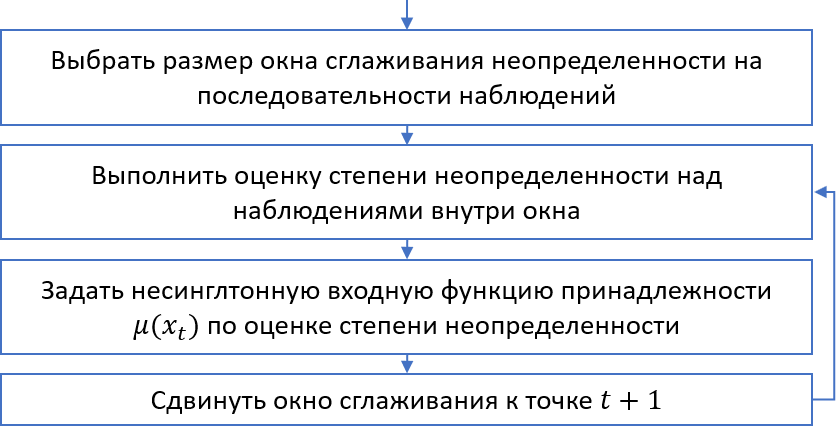
\includegraphics[width=0.8\textwidth]{ns-procedure}
	\caption{Схема обобщенной процедуры адаптивной несинглтонной фаззификации временной последовательности.}
	\label{fig:ns-procedure}
\end{figure}

\begin{figure}[thb]
\centering
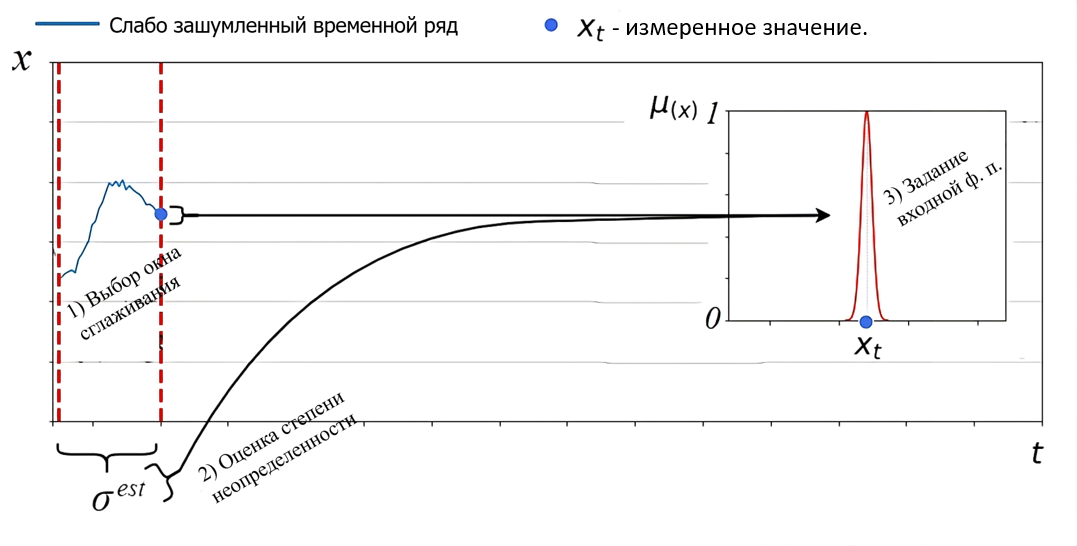
\includegraphics[width=0.9\textwidth]{ns-demo-low-noise}
\caption{Иллюстрация процедуры несинглтонной фаззификации временного ряда с низким уровнем шума.}
\label{fig:ns-demo-low-noise}
\end{figure}

\begin{enumerate}
	\item \textit{Выбрать размер окна сглаживания:} Определяется размер окрестности точки во временном ряде, по которому выполняется оценка степени неопределенности в точке. Размер окна может быть фиксированным или динамическим (например, при использовании экспоненциально взвешенного скользящего среднего). Например, при использовании датчиков (например, в робототехнике)	размер окна может быть выбран в зависимости от частоты съема датчиков или на основе фиксированного временного интервала. Другой подход, например, в контексте	временных рядов, может заключаться в использовании алгоритма подбора для определения оптимального размера окна.
	\item \textit{Оценить степень неопределенности внутри окна:} Теперь для оценки степени неопределенности в точке используется сформированный набор наблюдений временной последовательности. В зависимости от условий эксперимента, могут использоваться различные техники оценки неопределенности: статистическая (дисперсия), максимальное правдоподобие, глубокие нейросетевые автоэнкодеры, метод главных компонент \todo{добавить ссылки}. 
	\item \textit{Задать функцию принадлежности входного нечеткого множества:} Используя оценку степени неопределенности из предыдущего шага, следует задать параметры функции принадлежности входного нечеткого множества, то есть, выполнить непосредственно фаззификацию.
	\item \textit{Сдвинуть окно сглаживания:} Затем следует выполнить оценку степени неопределенности и фаззификацию для точки, следующей за текущей.
\end{enumerate}

На рисунке \cref{fig:ns-demo-low-noise} изображено как каждое несинглтонное входное нечеткое множество задается на основе оценки уровня шума, определенного по описанной только что процедуре с применением скользящего окна сглаживания. На этом рисунке показан участок наблюдений с низким уровнем шума приводящий к узкой ширине (среднеквадратичному отклонению) ф. п. входного нечеткого множества. На рисунке \cref{fig:ns-demo-large-noise} уровень шума заметно больше и, как следствие, ф. п. входного нечеткого множества имеет большую ширину.

\begin{figure}[bth]
	\centering
	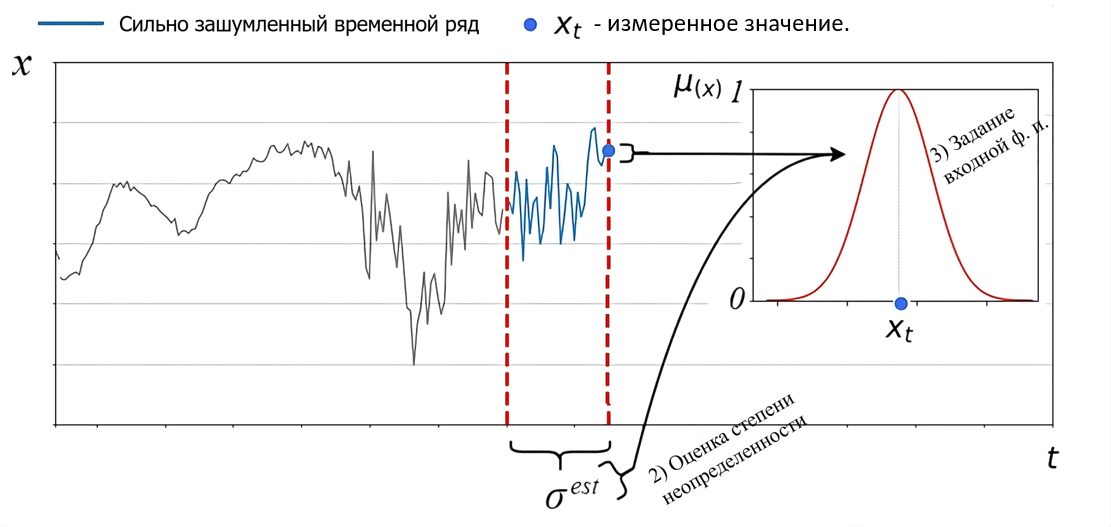
\includegraphics[width=0.9\textwidth]{ns-demo-large-noise}
	\caption{Иллюстрация процедуры несинглтонной фаззификации временного ряда с высоким уровнем шума.}
	\label{fig:ns-demo-large-noise}
\end{figure}

\subsection{Описание нечеткой модели прогнозирования временных рядов на основе нечеткого значения истинности}

Для временного ряда $\mathbf{y_t} = (y_1, \dots, y_T)$, где $T$ --- длина временной последовательности, величина $y_t$ представляет измеренное значение наблюдаемой переменной в момент времени $t=\overline{1,T}$. Ставится задача предсказания значений $\hat{y}_{t+h}$ для заданного горизонта прогнозирования $h$.

Модель временного ряда $f(\cdot)$ порядка $p$ использует последние $p$ значений до момента $t$ для оценки значения:
\[
\hat{y}_{t+h} = f(y_{t-p}, \dots, y_t),
\]
где $p$ - размер окна запаздывания.

При моделировании временных последовательностей с использованием нейро-нечетких систем каждое значение $y_t\in Y$ фаззифицируется в нечеткое множество $A_t$. Эти нечеткие множества составляют множество термов лингвистической переменной $y_t$ со значениями, определенными на базовом множестве $Y$. Такая система принимает $p$ входов, а правила в ее базе знаний устанавливают нечеткую последовательно-временную связь между заданным окном запаздывания размера $p$ и значением временного ряда в момент $t+h$. Параметр $p$ называется порядком нечеткой системы прогнозирования временных рядов.

База правил в такой системе представляется набором из $N$ правил вида:
\begin{equation}
	\begin{aligned}
		R_k: \textrm{Если }&y_{t-p}\textrm{ есть }A_{k1}\textrm{ и }\dots\textrm{ и } y_{t}\textrm{ есть }A_{kp},&\\
		\textrm{ то }&y_{t+h}\textrm{ есть }A_{k\,p+h},&k\in\overline{1,N},
	\end{aligned}
	\label{eqn:fts-rules}
\end{equation}
где каждое нечеткое отношение $\mathrm{T_1}\left\{A_{k1}, \dots, A_{kp}\right\} \rightarrow A_{k\,p+1}$, заданное в правиле $R_k$, выражает единицу \todo{логических} знаний о моделируемом протекающем во времени процессе.


\subsection{Построение базы правил}

Для построения базы правил у популярных в литературе типов нечетких систем Мамдани и Такаги-Сугено широко применяется алгоритм формирования правил но из данных \cite{Wang1992}. В контексте задачи прогнозирования временных рядов широкое применение в публикациях получили различные методы, являющиеся развитием или продолжением данного алгоритма \cite{Chellai2022}.

В этих подходах нечеткие множества, задающие значения в правилах, интерпретируются как термы лингвистических переменных. В контексте временных рядов это означает, что область значений изменяющейся во времени величины разбивается на соседствующие отсчеты (интервалы), каждому из которых соответствует терм лингвистической переменной.

\begin{enumerate}
	\item Границы пространство значений временной последовательности $U = [D_{min} - \delta_1, D_{max} + \delta_2]$ задаются на основе минимального $D_{min}$ и максимального $D_{max}$ присутствующих в данных значений с некоторыми отступами $\delta_1$ и $\delta_2$ соответственно.
	\item Пространство $U$ разбивается на $m$ равных отсчетов $u_1, u_2, \dots, u_m$.
	\item Набор соответствующих отсчетам нечетких множеств формирует множество термов лингвистических переменных $y_t, t=\overline{1, T}$.
	\item Затем каждому измеренному значению ставится в соответствие терм лингвистической переменной с наибольшей степенью истинности. Из последовательностей таких термов формируется набор правил --- набор нечетких отношений.
\end{enumerate}

Очевидным недостатком такого примитивного способа разбиения пространства значений является несоответствие часто отличному от равномерного распределению функции плотности вероятности этих значений. База правил формировалась напрямую из экземпляров данных, посредством сопоставления каждому экземпляру комбинации термов, имеющих наибольшую степень принадлежности по входам в совокупности.

%Развитие способов обучения нечетких систем в рамках задачи прогнозирования временных рядов проходило взаимосвязано с адаптацией нечеткого моделирования как непосредственно к задаче регрессии временных рядов, так и к задачам моделирования другого рода. Ранние подходы следовали более типовому набору шагов при построении нечетких систем \cite{Chellai2022}. При формирования набора термов лингвистической переменной $\tilde{y}$ ее пространство значений ограничивалось минимальным и максимальными значениями временного ряда и разбивалось на накладывающиеся друг на друга участки, каждый из которых составлял носитель соответствующего нечеткого множества из набора термов. В широко цитируемом подходе Chen-а \cite{Chen1996} разбиение производилось на равные отрезки. Очевидным недостатком такого примитивного способа разбиения пространства значений является несоответствие часто отличному от равномерного распределению функции плотности вероятности этих значений. База правил формировалась напрямую из экземпляров данных, посредством сопоставления каждому экземпляру комбинации термов, имеющих наибольшую степень принадлежности по входам в совокупности, что соответствует довольно популярному из-за своей простоты методу Wang-а \cite{Wang1992}. Такой способ построения базы правил нечеткой системы до сих пор популярен при исследовании нечетких моделей временных рядов и других данных, когда необходимо сравнить качество непосредственно моделирования при том же наборе данных и способе построения базы правил.

%В более поздних способах стало более распространенным формирование базы правил с соответствующими терм-множествами из данных, то есть подбор параметров функций принадлежности термов выполняется одновременно с формированием набора правил. Этот подходя является более простым и точным для выделение шаблонных отрезков из временных рядов, особенно в случаях сложной функции плотности распределения значений временного ряда, когда проявляются ограничения в увеличении точности нечеткой системы при разбиения базового множества лингвистической переменной $\tilde{y}$. Таким образом одни и те же методы можно применять для разбиения пространства значений временных рядов (одно измерение) или для разделения пространства окон временных рядов (когда последовательность значений в окне временного ряда интерпретируется как точка в $n$-мерном пространстве). В последнем случае посредством разбиения пространства окон временного ряда может осуществляться формирование базы правил.

%Распространенной группой таких методов являются подходы на основе различных алгоритмов кластеризации \cite{Lucas2021}:  \textit{k}-средних, алгоритмы учитывающие плотность распределения точек, агломеративная кластеризация.

%Эволюционные подходы, например, Particle Swarm Optimization (PSO)\cite{Davari2009} могут обеспечить оптимальную настройку параметров нечеткой модели при сложной конфигурации обучающего набора данных. 

%Основная сложность использования этих методов состоит в необходимости выполнять большое количество вычислений функции приспособленности на всем обучающем наборе данных на каждой итерации для всех особей популяции. Поэтому для сокращения времени оценки параметров модели стараются минимизировать набор параметров, для которых применяются методы глобальной оптимизации.

Чаще используются подходы построения базы правил, где значения термов в каждом правиле являются индивидуальным, то есть подбираются параметры нечетких множеств в правилах с уходом от лингвистической интерпретации.

Тогда каждое такое нечеткое множество в каждом правиле будет определяться индивидуальными значениями параметров функции принадлежности, а для задания всей базы правил требуется задание матрицы параметров $\theta_{\mathbf{R}}$

\begin{equation*}
	\theta_{\mathbf{R}} = \begin{bmatrix}
		\theta_{\mu_{\mathbf{R_1}}}\\
		\vdots\\
		\theta_{\mu_{\mathbf{R_N}}}
	\end{bmatrix} = \begin{bmatrix}
		\theta_{\mu_{A_{11}}} & \theta_{\mu_{A_{12}}} & \dots & \theta_{\mu_{A_{1n}}} & \theta_{\mu_{B_{1}}} \\
		\vdots & \vdots & \ddots & \vdots & \vdots \\
		\theta_{\mu_{A_{N1}}} & \theta_{\mu_{A_{N2}}} & \dots & \theta_{\mu_{A_{Nn}}} & \theta_{\mu_{B_{N}}} \\
	\end{bmatrix}.
\end{equation*}

При использовании гауссовых функций принадлежности c параметрами $a$ и $b$ для нечетких множеств в правилах матрица параметров может быть записана следующим образом:

\begin{equation*}
	\theta_{\mathbf{R}} = \begin{bmatrix}
		\langle a_{\mu_{A_{11}}}, b_{\mu_{A_{11}}}\rangle & \langle a_{\mu_{A_{12}}}, b_{\mu_{A_{12}}}\rangle & \dots & \langle a_{\mu_{A_{1n}}}, b_{\mu_{A_{1n}}}\rangle & \langle a_{\mu_{B_{1}}}, b_{\mu_{B_{1}}}\rangle \\
		\vdots & \vdots & \ddots & \vdots & \vdots \\
		\langle a_{\mu_{A_{N1}}}, b_{\mu_{A_{N1}}}\rangle & \langle a_{\mu_{A_{N2}}}, b_{\mu_{A_{N2}}}\rangle & \dots & \langle a_{\mu_{A_{Nn}}}, b_{\mu_{A_{Nn}}}\rangle & \langle a_{\mu_{B_{N}}}, b_{\mu_{B_{N}}}\rangle \\
	\end{bmatrix}.
\end{equation*}

Для подбора параметров функций принадлежности в наборе правил используется оптимизация этих параметров на основе набора данных, а критерием оптимизации является минимизация метрики среднеквадратичной ошибки (RMAE - Root Mean Square Error). В качестве такого алгоритма выбран \textit{метод роя частиц (Particle Swarm Optimization - PSO)}, который приведен на рисунке Алгоритм \ref{alg:pso}. Частицы в PSO используют как собственный опыт, так и опыт соседей, сглаживая свою траекторию за счет использования промежуточного вектора скорости для каждой точки, дающего эффект инерции. Это позволяет алгоритму избегать застревания в локальных минимумах. В контексте оптимизации вектора параметров функций принадлежности базы правил большой размерности (часто, сотни параметров), PSO хорошо выполняет оптимизацию по всем размерностям одновременно. При работе алгоритм сперва исследует широкое пространство решений, а затем сосредоточиться на его уточнении, что также позволяет бороться с попаданием в локальный оптимум. Основные параметры --- количество частиц $S$, вес инерции $\omega$ и коэффициенты влияния текущего локального $\phi_l$ и глобального $\phi_g$ оптимума.

\begin{algorithm}[p]
	\caption{Particle Swarm Optimization (PSO) для подбора параметров ф. п. в правилах на основе эталонных данных}
	\label{alg:pso}
	\begin{algorithmic}[1]
		\Require
		\Statex $S$ --- количество частиц
		\Statex $max\_iter$ --- количество итераций
		\Statex $\omega$ --- вес инерции
		\Statex $\phi_l, \phi_g$ --- коэффициенты влияния локального и глобального оптимума
		\Statex $b_{lo}, b_{up}$ --- вектора нижних и верхних граничных значений вектора параметров частицы $\theta_p$
		\Statex $D_{l=1}^M$ --- набор эталонных данных
		\Statex $f(\theta)$ --- целевая функция приспособленности для набора данных $D$
		
		\Statex \textbf{Инициализация:}
		\For{каждой частицы $p = 1, \dots, S$}
		\State Инициализировать позицию частицы по равномерному распределению: $\theta_p \sim U(b_{lo}, b_{up})$
		\State Установить $\theta^l_p \gets \theta_p$ \Comment{Локальный оптимум частицы}
		\State Инициализировать скорость по равномерному распределению: $v_p \sim U(-|b_{up}-b_{lo}|, |b_{up}-b_{lo}|)$ \Comment{Вектор скорости $v_p$ имеет такую же размерность как и вектор параметров $\theta_p$}
		\EndFor		
		\State $\theta^g \gets \argmin_{p} f(\theta^l_p)$ \Comment{Инициализация глобального оптимума}
		
		\Statex \textbf{Основной цикл:}
		\For{$i = 1, \dots, max\_iter$}
		\For{каждой частицы $p = 1, \dots, S$}
		\State Сгенерировать случайные $r_l, r_g \sim U(0,1)$
		\State Обновить скорость:
		\State \quad $v_p \gets \omega v_p + \phi_l r_l (\theta^l_p - \theta_p) + \phi_g r_g (\theta^g - \theta_p)$
		\State Обновить позицию:  $\theta_p \gets \theta_p + v_p$
		\If{$f(\theta_p) < f(\theta^l_p)$}
		\State Обновить локальный оптимум: $\theta^l_p \gets \theta_p$
		\If{$f(\theta^l_p) < f(\theta^g)$}
		\State Обновить глобальный оптимум: $\theta^g \gets \theta^l_p$
		\EndIf
		\EndIf
		\EndFor
		\EndFor
		
		\State \textbf{Возврат} $\theta^g$ \Comment{Найденный глобальный оптимум}
	\end{algorithmic}
\end{algorithm}

\section{Постановка задачи}

\section{Применение нечекого значения истинности}

Определив НЗИ $CP(\mathbf{A_{k}, \mathbf{A'}})$ для антецедента правила $R_k$ согласно (\ref{eqn:ftv-compute-12}) и (\ref{eqn:ftv-compute-8}), можно переписать правило $R_k$ в виде:
\begin{align*}
	R_k: \textrm{Если }&CP(\mathbf{A_{k}, \mathbf{A'}}),&\\
	\textrm{ то }&y_{t+1}\textrm{ есть }A_{k\,p+1},&k\in\overline{1,N}.
\end{align*}


\section{Описание вычислительного эксперимента для оценки характеристик применения разработанного метода к задаче регрессии временных рядов}

Для подтверждения утверждения о полиномиальной (линейной) временной сложности нечеткого вывода на основе нечеткого значения истинности и провести сравнение использования логического нечеткого вывода Л. Заде в задаче, где актуален учет нечеткости данных, с подходами Мамдани и Такаги-Сугено, следует провести несколько вычислительных экспериментов и выполнить оценку характеристик разработанного подхода в этой задаче.

Для простоты сравнения с результатами публикаций, использующих несинглтонную фаззификацию, для проведения экспериментов будет использоваться синтетический набор данных Mackey-Glass (M-G). Набор данных с такими же значениями параметров уравнения, как в этих публикациях: $\tau = 30, \beta = 0.2, \gamma = 0.1$. Так же была сгенерирована последовательность из 2000 точек на участке от $t=-999$ до $t=1000$. Первые 1000 точек так же выбрасываются как зона стабилизации процесса $x(t)$, а следующие $T=1000$ точек на участке $t=\overline{1,1000}$ используются в эксперименте.

\begin{equation}
	\frac{dx(t)}{dt} = \beta\frac{x(t-\tau)}{1+x(t-\tau)^n}-\gamma x(t)
	\label{eqn:mackey-glass-definition}
\end{equation}


В данном эксперименте используется адаптивный метод оценки зашумленности в точке $t$ временной последовательности. Для этого сперва вычисляется последовательность разностей $d_t$ соседних значений временной последовательности (\ref{eqn:mackey-glass-definition}).

\begin{align}
	\label{eqn:mackey-glass-seq-diff}
	d_1 &= d_2, \\
	d_t &= \frac{1}{\sqrt{2}}(x_t - x_{t-1}),
\end{align}
где $t\in[1;T]$.

А затем для каждой точки вычисляются значения среднеквадратичных отклонений $\hat{\sigma}_t$ разностей соседних точек (\ref{eqn:mackey-glass-seq-diff-std}), но, в отличии от \cite{Pekaslan2020}, вычисление производится не внутри скользящего окна фиксированного размера, а на основе формулы экспоненциально взвешенного скользящего среднего:

\begin{align}
	\hat{\sigma}^2_t &= (1-\alpha) \hat{\sigma}^2_{t-1} + \alpha (d_t - \hat{d}_t) \notag \\
			  		 &= \sum_{p=1}^t \alpha (1-\alpha)^{t-p} (d_p - \hat{d}_p)^2, \label{eqn:mackey-glass-seq-diff-var-iterative} \\
	\hat{\sigma}_t &= \sqrt{\hat{\sigma}^2_t}, \label{eqn:mackey-glass-seq-diff-std}
\end{align}
где $\hat{d}_t$ --- является экспоненциально взвешенным скользящим средним значений $d_t$:
\begin{align}
	\hat{d}_t &= (1-\alpha) \hat{d}_{t-1} + \alpha d_t \notag \\
	&= \sum_{p=1}^t \alpha (1-\alpha)^{t-p} d_p. %\notag
	\label{eqn:mackey-glass-seq-diff-mean}
\end{align}

Таким образом, в данном способе оценки уровня шума в измеренных значениях \cite{Rank1999} сперва с помощью разностного оператора выполняется преобразование в стационарный временной ряд (исключение компоненты тренда) для более точной оценки амплитуды шума, а затем среднеквадратичное отклонение в экспоненциально взвешенной области отражает резкие изменения значений стационарного временного ряда относительно сглаженного центра в данной точке $t$.

\begin{figure}[ht]
	\centering
	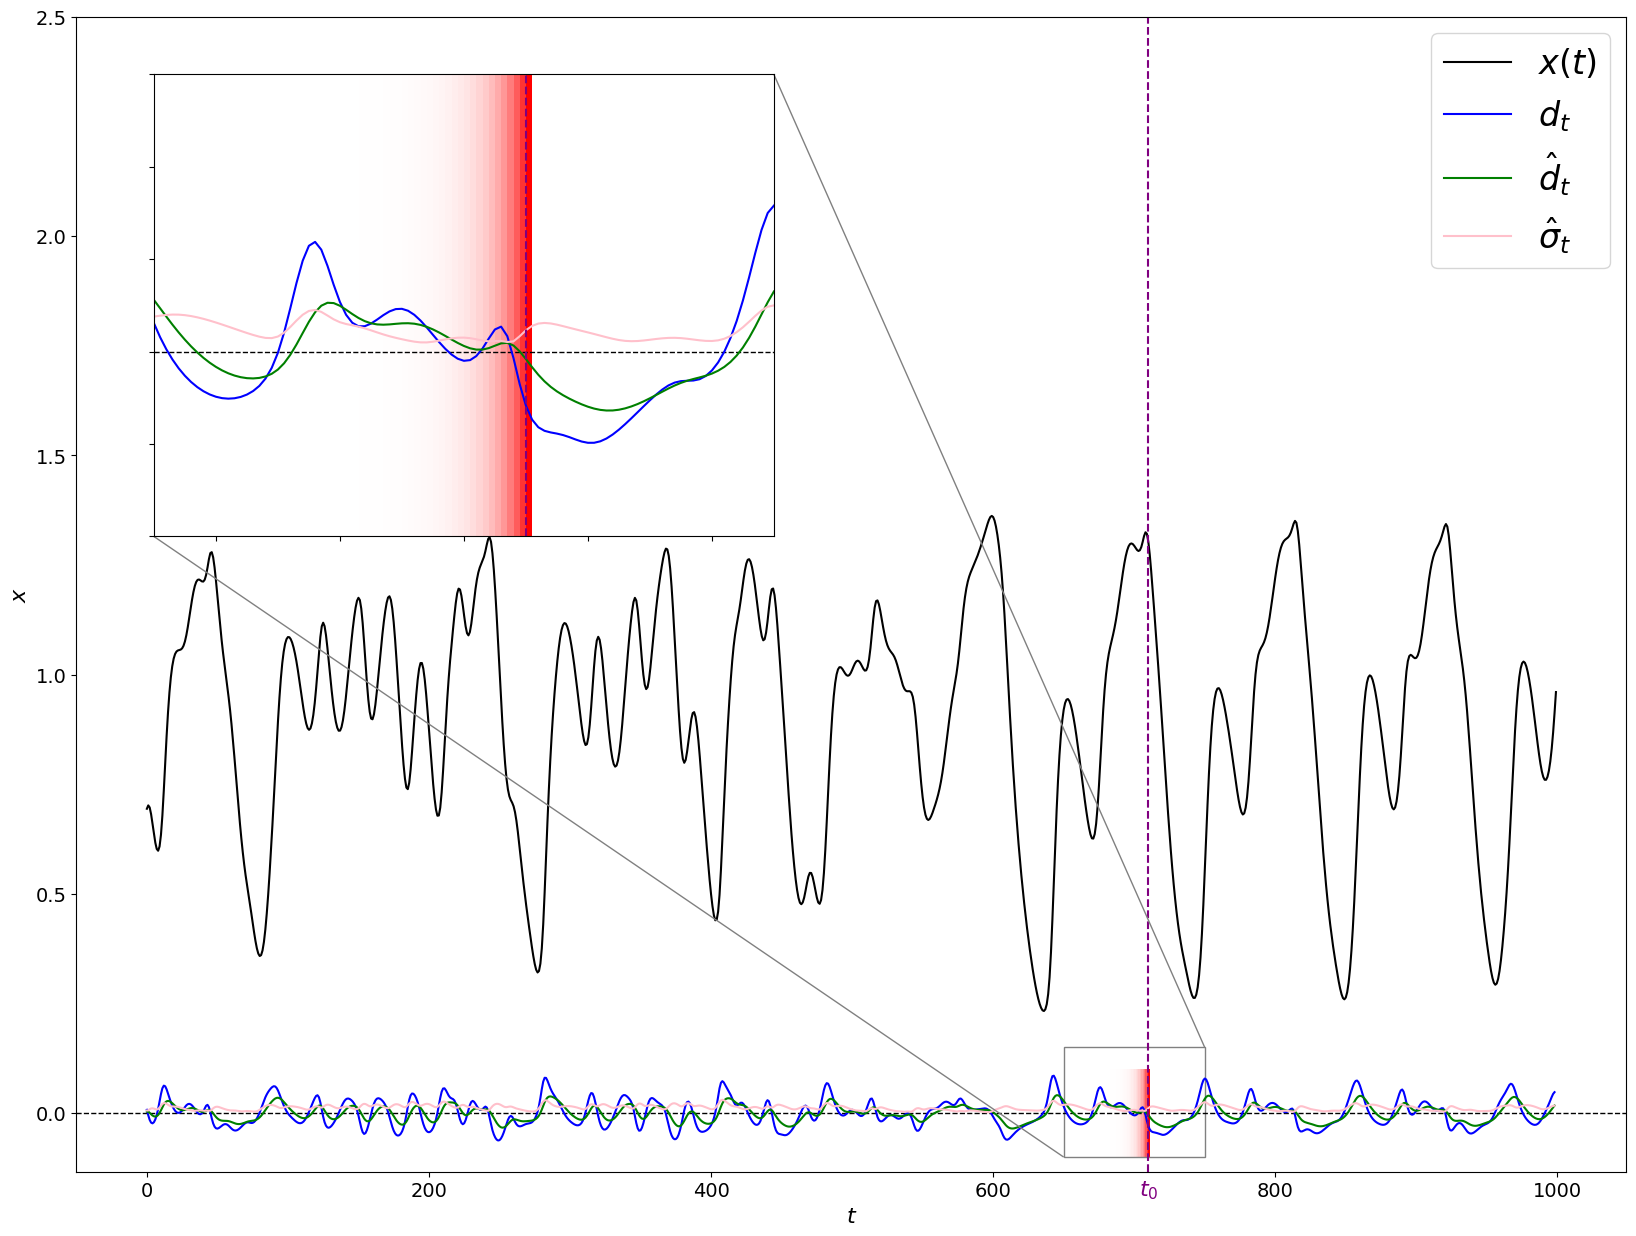
\includegraphics[scale=0.3]{mackey-glass-ewma-example}
	\caption{График сгенерированной последовательности Mackey-Glass $x(t), t\in[0;999]$ с параметрами $\tau = 30, \beta = 0.2, \gamma = 0.1$, график разностей соседних точек $d_t$ последовательности $x(t)$, график $\hat{d}_t$ с наложением экспоненциально взвешенного сглаживания на последовательность разностей и график экспоненциально взвешенного скользящего среднеквадратичного отклонения разностей $\hat{\sigma}_t$. На вложенном изображении участка $t\in[650,750]$ яркостью красного цвета показано значения весового коэффициента $\alpha (1-\alpha)^{t-p}, p=\overline{1,t_0}$ из формулы (\ref{eqn:mackey-glass-seq-diff-var-iterative}) при $\alpha = 0.2$, определяющего степень вклада предыдущих значений $(d_p - \hat{d}_p)^2$ в значение $\hat{\sigma}^2_t$ в точке $t$. Чем меньше значение $\alpha$, тем слабее <<доверие>> к одному лишь значению $d_t$ и тем больше предыдущих значений $d_p$ делают вклад в сглаженное значение.}
	\label{fig:mackey-glass-ewma-example}
\end{figure}

Для каждого значения временной последовательности $x(t)$ в результате фаззификации было получено нечеткое множество $A'_t$ с гауссовой функцией принадлежности с параметрами $a$ и $b$:
\begin{equation*}
	\begin{aligned}
		\mu_{A'_t}(y_t) &= gauss(y_t; a, b), \\
		\theta_{\mu_{A'_t}} &= \langle a, b \rangle = \langle x(t), \phi\,\hat{\sigma}_t\rangle,
	\end{aligned}
\end{equation*}
где параметр среднеквадратичного отклонения равен ранее вычисленному значению $\hat{\sigma}_t$ с коэффициентом $\phi = 0.3$.



Для построения базы правил использовались точек в диапазоне от $t=1$ до $t=700$ (обучающий диапазон) из ранее отложенных $T=1000$ точек, а для оценки качества итоговой системы были взяты последние 300 точек в диапазоне от $t=701$ до $t=1000$ (тестовый диапазон). Диапазоны последовательности этих точек были составлены обучающий и тестовый наборы временных отрезков длины $p+1$ с использованием скользящего окна, где размер окна запаздывания $p$ выбирался среди значений $3,5,7,9,11$, а горизонт прогнозирования установлен $h=1$. В нечетком выводе использовалась импликация Лукасевича, T-нормы --- min и метода дефаззификации средний максимум (MeOM) с количеством точек алгоритма Gradient-aware PSO --- 100 и количеством итераций --- 100.

Конфигурация вычислительной системы: центральный процессор --- AMD Ryzen 9 5900HX (8 ядер, 16 потоков, базовая частота 3.3 ГГц, кэш L3 16 МБ); оперативная память --- 32 ГБ DDR4-3200 (двухканальный режим); графический процессор --- NVIDIA GeForce RTX 3080 Laptop GPU с 16 ГБ видеопамяти (CUDA 12.1, compute capability --- 8.6).

\begin{figure}
	\centering
	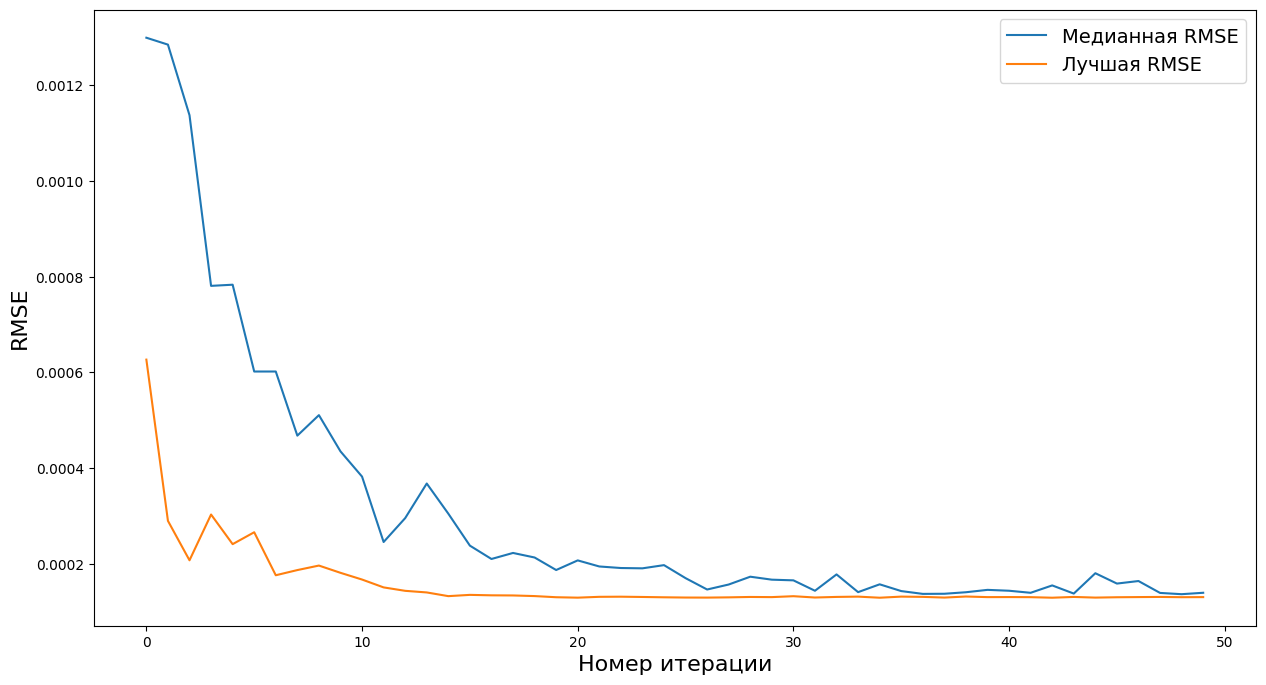
\includegraphics[scale=0.37]{mackey-glass-pso-optimization}
	\caption{Графики изменений среднего и лучшего по популяции значений оптимизируемой функции приспособленности при числе входов нечеткой системы ---7, количестве правил --- 20, размере набора точек алгоритма PSO --- 50 и количестве итераций --- 50.}
	\label{fig:mackey-glass-pso-optimization}
\end{figure}

Динамика среднего (медианного) и лучшего по набору точек значений оптимизируемой метрики в процессе PSO-оптимизации базы правил для указанных выше значений набора гиперпараметров изображена на рисунке \cref{fig:mackey-glass-pso-optimization}.

\begin{figure}
	\centering
	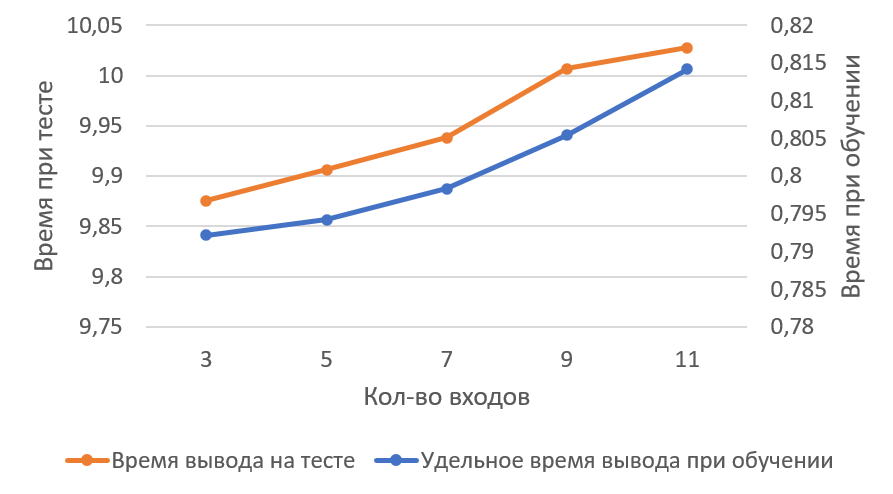
\includegraphics[scale=0.7]{mackey-glass-inference-duration}
	\caption{График длительности выполнения параллельной реализации нечеткого вывода для обучающего и тестового набора данных при количестве правил $N=10$.}
	\label{fig:mackey-glass-inference-duration}
\end{figure}

После проведенного вычислительного эксперимента были получены показатели удельного (на одну точку из набора точек одной итерации алгоритма PSO) времени работы алгоритма нечеткого вывода на основе НЗИ на обучающем наборе данных и времени работы на тренировочном наборе данных для различного размера окна запаздывания, изображенные на рисунке \cref{fig:mackey-glass-inference-duration}. На этом рисунке наблюдается линейный рост времени выполнения алгоритма с увеличением количества входов нечеткой системы, что \textbf{подтверждает утверждение о полиномиальной зависимости временной сложности метода нечеткого вывода на основе НЗИ от количества входов}. Временные показатели алгоритма нечеткого вывода для тестового набора данных также включают значительную временную компоненту задержки, вызванную в основном процессом инициализации библиотек при первичном запуске нечеткого вывода для уже готового набора правил, тогда как на обучающем наборе данных получены значения времени работы непосредственно алгоритма нечеткого вывода с амортизированной компонентой задержки.

\begin{figure}
	\centering
	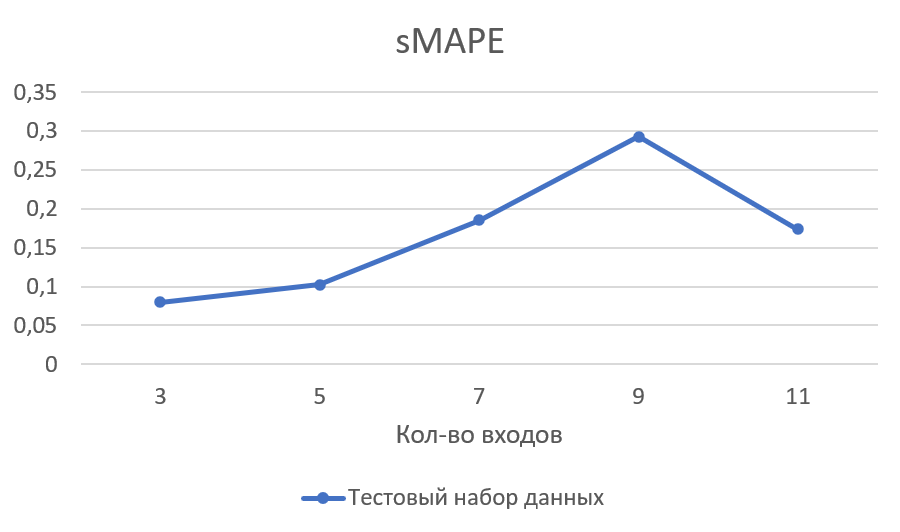
\includegraphics[scale=0.7]{mackey-glass-inference-smape}
	\caption{График значений метрики sMAPE на обучающем и тестовом наборах данных при различных размерах окна запаздывания, количестве правил --- 30.}
	\label{fig:mackey-glass-inference-smape}
\end{figure}

С целью сравнения с альтернативными нечеткими моделями на примере решения этой же задачи при наиболее близких условиях для полученной в результате экспериментов нечеткой системы затем выполнена оценка точности прогнозирования по метрике \textit{Symmetric Mean Absolute Percentage Error (sMAPE)}, определяемой формулой:
\[
sMAPE = \frac{100\%}{n} \sum_{t=1}^n 
\frac{|y_t - \hat{y}_t|}{\tfrac{|y_t| + |\hat{y}_t|}{2}},
\]
где $y_t$ и $\hat{y}_t$ соответствуют истинному и предсказанному значению в момент времени $t$.




Значение этой метрики для разных размеров окна запаздывания приведены на рисунке \cref{fig:mackey-glass-inference-smape}, где лучший показатель качества прогнозирования временного ряда по метрике sMAPE достигается при размере окна запаздывания --- 3 точки. Тогда соответствующая матрица параметров базы правил имеет вид размера $30\times 4$:
\begin{equation*}
	\theta^*_{\mathbf{R}} = \begin{bmatrix}
		\langle a_{\mu_{A_{1\,1}}}, b_{\mu_{A_{1\,1}}}\rangle & \langle a_{\mu_{A_{1\,2}}}, b_{\mu_{A_{1\,2}}}\rangle & \langle a_{\mu_{A_{1\,3}}}, b_{\mu_{A_{1\,3}}}\rangle & \langle a_{\mu_{B_{1}}}, b_{\mu_{B_{1}}}\rangle \\
		\vdots & \vdots & \vdots & \vdots \\
		\langle a_{\mu_{A_{30\,1}}}, b_{\mu_{A_{30\,1}}}\rangle & \langle a_{\mu_{A_{30\,2}}}, b_{\mu_{A_{30\,2}}}\rangle & \langle a_{\mu_{A_{30\,3}}}, b_{\mu_{A_{30\,3}}}\rangle & \langle a_{\mu_{B_{30}}}, b_{\mu_{B_{30}}}\rangle \\
	\end{bmatrix}.
\end{equation*}

Достигнутое в этом случае значение $sMAPE = 8\%$ при количестве правил 30, заметно превосходит точность моделирования незашумленной последовательности Mackey-Glass (M-G) с использованием синглтонной фаззификации со значением $sMAPE \approx 40\%$ в \cite{Pekaslan2020}. Также полученное качество прогнозирования сопоставимо со значением этой метрики при аналогичной конфигурации эксперимента прогнозирования временного ряда M-G в той же публикации, где для достижения точности моделирования временной последовательности $sMAPE \approx 10\%$ используется нечеткая система типа Мамдани, содержащая 184 правила\footnote{Непосредственно в самой статье не указано количество используемых правил. Однако авторами этой статьи опубликован программный код описанного в статье метода, запустив который удалось воспроизвести проводимые авторами эксперименты и восстановить количество правил в их нечетких системах.} в базе правил для не зашумленного временного ряда M-G и 597, 402, 312 правил для различных конфигураций и амплитуды добавленного шума. Данные наблюдения показывают, что \textbf{метод регрессии временных рядов на основе логического нечеткого вывода при несинглтонной фаззификации значительно превосходит качество регрессии с использованием синглтонной фаззификации, а также имеет сопоставимую с методом регрессии Мамдани при несинглтонной фаззификации точность, но при меньшем количестве правил} за счет возможности построения более сложной функции аппроксимации.

\section{Применение разработанной нечеткой модели в задаче прогнозирования объема транзакций по безналичным платежам для клиентов банка}

Теперь применим разработанную модель для решения задачи прогнозирования временной последовательности в прикладной области для сравнительной оценки качества прогнозирования данной нечеткой моделью с другими подходами в этой задаче.

Была выбрана задаче прогнозирования помесячной транзакционной активности (объема транзакций) клиентов банка по одному из продуктов банка --- безналичные платежи (более распространенное название --- эквайринг). Данная услуга банка позволяет юридическим лицам принимать безналичные платежи от своих клиентов с помощью банковских карт и других платежных систем, таких как мобильные платежи (например, Mir Pay, Google Pay, Apple Pay) или QR-коды. Различные виды безналичной оплаты продемонстрированы на рисунке \cref{fig:acquiring-examples}. Каждая разновидность способа безналичной оплаты соответствует отдельному типу транзакций.

\begin{figure}[t]
	\centering
	\begin{minipage}[b][][b]{0.3\textwidth}
		\centering
		
\includegraphics[height=3.5cm]{acquiring-pos-terminal} \\ POS-терминал
		%\caption*{POS-терминал}
	\end{minipage}
	%\hfill %\hspace{0.02\textwidth}
	\begin{minipage}[b][][b]{0.33\textwidth}
		\centering
		
\includegraphics[height=3.5cm]{acquiring-internet} \\ Интернет-эквайринг
		%\caption*{Интернет-эквайринг}
	\end{minipage}
	%\hfill %\hspace{0.02\textwidth}
	\begin{minipage}[b][][b]{0.3\textwidth}
		\centering
		
\includegraphics[height=3.5cm]{acquiring-qr-code} \\ QR-код
		%\caption*{QR-код}
	\end{minipage}
	\vfill
	\caption{Различные виды безналичной оплаты.}
	\label{fig:acquiring-examples}
\end{figure}

\todo{Описать бизнес-смысл построения прогноза по данному продукту}

Временной ряд клиента в этом наборе данных имеет вид помесячных значений объемов транзакций $s_t$, каждое из которых получено в результате агрегации (складывания) сумм отдельных транзакций $x_{t\,i}$ за месяц:
\begin{equation*}
	s_t = \sum_{i=1}^{N_t} x_{t\,i},
\end{equation*}
где $N_t$ --- количество транзакций за месяц $t$.

%Сумма каждой транзакции $x_{t\,i}$ является полностью четким достоверным значением и, как следствие, помесячные агрегации $s_t$ являются четкими значениями, не подверженными шумовому воздействия или другой неопределенности непосредственно самих значений месячных объемов транзакций. Однако, в зависимости от рода деятельности клиента банка, сам временной ряд может иметь разную степень стохастичности, возникающей из-за скрытой многофакторной неопределенности при деятельности клиента, отражающейся в размере волатильности (динамики изменчивости объема) цепочки отдельных транзакций.
%
%Волатильность временного ряда в точке $t$ можно оценить с помощью описанного в предыдущем эксперименте метода оценки среднеквадратичного отклонения в точке $t$ \cite{} с использованием формул (\ref{eqn:mackey-glass-seq-diff}),  (\ref{eqn:mackey-glass-seq-diff-mean}), (\ref{eqn:mackey-glass-seq-diff-var-iterative}) и (\ref{eqn:mackey-glass-seq-diff-std}). Среднеквадратичное отклонение $\sigma_{s_t|N_t}$ временного ряда помесячных агрегаций в момент $t$ может быть выражено через среднеквадратичное отклонение $\sigma_{x_t}$ для $N_t$ отдельных транзакций внутри месяца c использованием соответствующих дисперсий:
%\begin{equation*}
%	\begin{aligned}
%		\sigma^2_{s_t|N_t} = N_t \sigma^2_{x_{t}}.\\
%	\end{aligned}
%\end{equation*}
%
%Тогда волатильность транзакций внутри месяца можно выразить:
%\begin{equation*}
%	\sigma_{x_t} = \sqrt{\frac{\sigma^2_{s_t|N_t}}{N_t}}
%\end{equation*}
%
%В \cite{Green2015} подмечено: при низкой волатильности --- более простые и плавные модели часто превосходят сложные, но с высокой волатильностью справляются только сложные модели с высокой емкостью знаний и учитывающие волатильность. Как было показано в первой главе при увеличении ширины функции принадлежности нечеткого множества входного значения увеличивается количество активируемых окрестных правил нечеткой системы. То есть при малой ширине входной ф. п. выходное значение получается в узкой области небольшого количества правил, а при большой ширине входной ф. п. задействуется большое количество правил в широкой области, то есть по сути повышается емкость нечеткой системы. Тогда волатильность объема транзакций внутри месяца $t$ может быть использована для задания ширины гауссовой функции принадлежности в процедуре фаззификации:
%\begin{equation*}
%	\begin{aligned}
%		\mu_{A'_t}(y_t) &= gauss(y_t; a, b), \\
%		\theta_{\mu_{A'_t}} &= \langle a, b \rangle = \langle s_t, \phi\,\sigma_{x_t}\rangle,
%	\end{aligned}
%\end{equation*}
%где коэффициент $\phi = 0.3$.

В зависимости от рода деятельности клиента банка, сам временной ряд может иметь разную степень стохастичности, возникающей из-за скрытой многофакторной неопределенности при деятельности клиента. Степень стохастичности временного ряда в точке $t$ можно оценить с помощью описанного в предыдущем эксперименте метода оценки среднеквадратичного отклонения в точке $t$ с использованием формул (\ref{eqn:mackey-glass-seq-diff}),  (\ref{eqn:mackey-glass-seq-diff-mean}), (\ref{eqn:mackey-glass-seq-diff-var-iterative}) и (\ref{eqn:mackey-glass-seq-diff-std}).

В \cite{Green2015} подмечено: для стабильных временных рядов --- более простые и плавные модели часто превосходят сложные, но с высокой степенью стохастичности справляются только сложные модели с большой емкостью знаний и учитывающие эту стохастичность. Как было показано в первой главе при увеличении ширины функции принадлежности нечеткого множества входного значения увеличивается количество активируемых окрестных правил нечеткой системы. То есть при малой ширине входной ф. п. выходное значение получается в узкой области небольшого количества правил, а при большой ширине входной ф. п. задействуется большое количество правил в широкой области, то есть по сути повышается емкость нечеткой системы. Тогда степень стохастичности месячного объема транзакций $t$ может быть использована для задания ширины гауссовой функции принадлежности в процедуре фаззификации:
\begin{equation*}
	\begin{aligned}
			\mu_{A'_t}(y_t) &= gauss(y_t; a, b), \\
			\theta_{\mu_{A'_t}} &= \langle a, b \rangle = \langle s_t, \phi\,\sigma_{s_t}\rangle,
		\end{aligned}
\end{equation*}
где коэффициент $\phi = 0.3$.

\begin{figure}[ht]
	\centering
	\begin{minipage}[b]{0.48\textwidth}
		\centering
		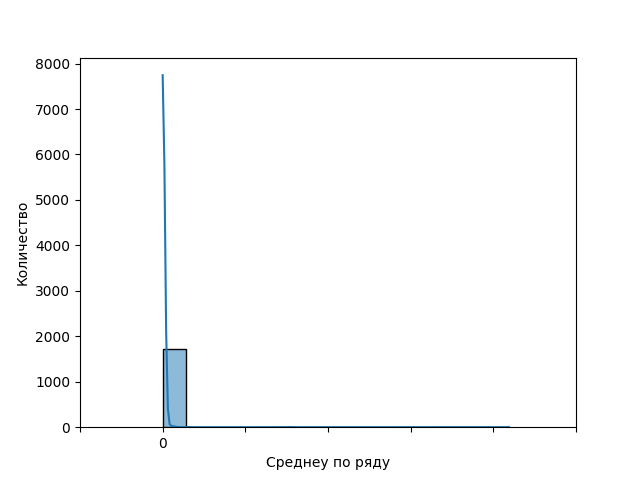
\includegraphics[width=\textwidth]{acquiring-values-hist}
		\caption*{Распределение значений $\Exp{s_t}$}
	\end{minipage}
	\hfill
	\begin{minipage}[b]{0.48\textwidth}
		\centering
		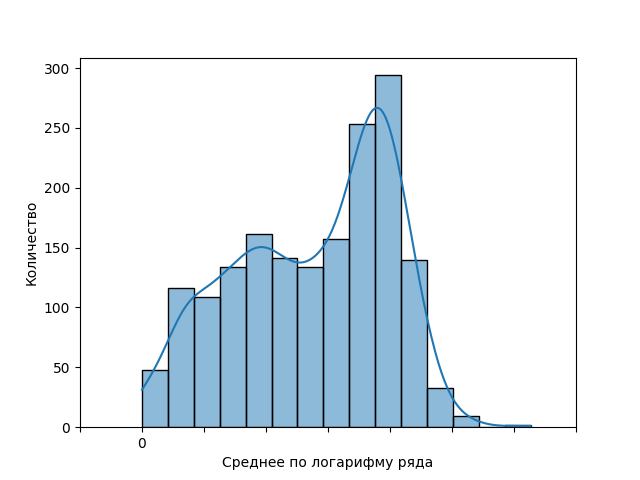
\includegraphics[width=\textwidth]{acquiring-log-hist}
		\caption*{Распределение значений $\Exp{\log{s_t}}$}
	\end{minipage}
	\caption{Гистограммы математических ожиданий временных рядов.}
	\label{fig:acquiring-values-hists}
\end{figure}

Исходный набор данных составлен из помесячных объемов транзакций за период с 01-01-2021 по 31-12-2023 для 2500 клиентов. Из набора данных были удалены временные ряды для клиентов, состоящие только из нулевых значений, то есть клиенты без активности по продукту банка. В результате остались временные ряды для 1731 активных клиентов. Образцы временных рядов приведены на рисунке \ref{}. Случайная величина средних по клиенту $\mathbb{E}[s_t]$ имеет экспоненциальное распределение, как показано на рисунке \cref{fig:acquiring-values-hists}. Для выравнивания этого распределения и для достижения более равномерного распределения пространства правил нечеткой системы было выполнено логарифмирование значений $s_t$ временных рядов.

\begin{figure}[ht]
	\centering
	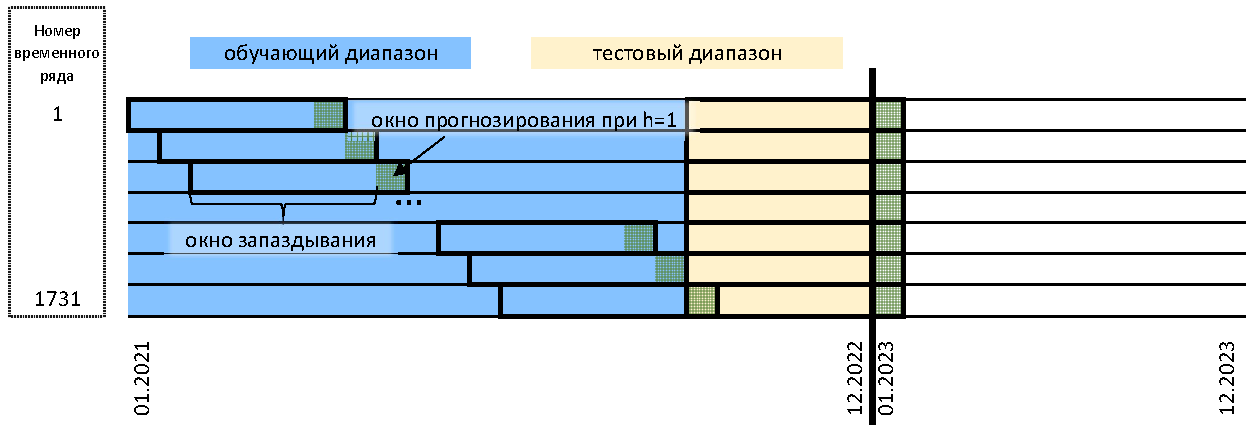
\includegraphics[scale=0.6]{acquiring-train-test-split}
	\caption{Разбиение временных рядов на обучающий и тестовый диапазоны.}
	\label{fig:acquiring-train-test-split}
\end{figure}

По требованиям задачи последние 12 месяцев были отложены в качестве прогнозируемых значений тестового диапазона, а период с 01-2021 по 12-2022 использовался в качестве обучающего диапазона для формирования набора обучающих окон с размером запаздывания $p = 3,6,9,12$ и горизонтом прогнозирования $h=1$ и $h=3$. Данный способ разбиения показан на рисунке \cref{fig:acquiring-train-test-split}. Для оценки качества прогнозирования использовалась целевая метрика RMAE, которая дает возможность сравнить насколько среднее значение ошибки высоко относительно среднего прогнозируемого значения:
\[
RMAE = \frac{MAE}{\mathbb{E}[\mathbb{E}[s_t]]} = \frac{\sum_{t=1}^n |y_t - \hat{y}_t|}{\sum_{t=1}^n y_t},
\]
где $y_t$ и $\hat{y}_t$ соответствуют истинному и предсказанному значению в момент времени $t$.

Обучение производилось при количестве правил нечеткой системы --- 50, точек PSO-алгоритма --- 50, количестве итераций --- 50. Как и в предыдущем эксперименте использовалась импликация Лукасевича и дефаззификация по среднему максимуму (MeOM) с теми же параметрами алгоритма Gradient-aware PSO. В качестве функции приспособленности выступала метрика среднеквадратичной ошибки (RMSE).

% \begin{figure}
% 	\centering
% 	%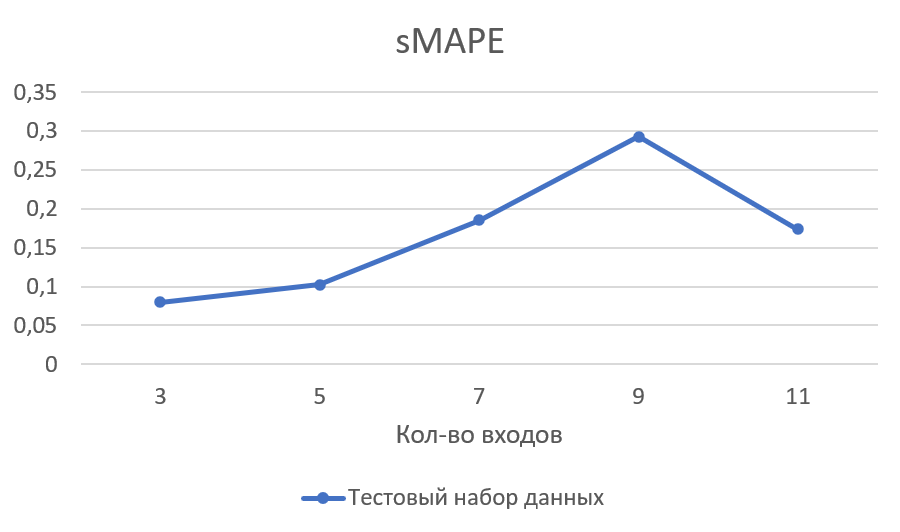
\includegraphics[scale=0.7]{mackey-glass-inference-smape}
% 	\caption{График значений метрики MAE на обучающем и тестовом наборах данных при различных размерах окна запаздывания, количестве правил --- 50.}
% 	\label{fig:acquiring-inference-mae}
% \end{figure}

Лучшее качество прогнозирования для разработанной модели NSFLS+FTV (Non-singleton Fuzzy Logical System с использованием Fuzzy Truth Value) удалось достичь при размере окна запаздывания --- 3 точки. Для сравнения с другими подходами, обычно применяемыми при решении такой задачи, в таблице \ref{tab:acquiring-metric-comparison} приведены значения метрики качества при прогнозирования на 1 и 3 месяца для моделей: наивная, ARIMA, градиентный бустинг, многослойный перцептрон, DeepAR. 

\begin{table}[t]
	\centering
	\begin{threeparttable}% выравнивание подписи по границам таблицы
		\caption{Значения метрики MAE относительно $\mathbb{E}[\mathbb{E}[s_t]]$ для разработанной NSFLS+FTV и альтернативных моделей.}%
		\label{tab:acquiring-metric-comparison}%
		\begin{tabular}{| c | c | c |}
			\toprule
			\multirow{2}{*}{Модель} & \multicolumn{2}{|c|}{Relative Mean Absolute Error (RMAE)} \\
			\cmidrule{2-3} & Прогноз на 1 мес. & Средняя за 3 мес. \\
			\midrule
			Наивная (среднее по ряду) & 0.166 & 0.204 \\
			ARIMA & 0.187 & 0.230  \\
			Градиентный бустинг & 0.152  & 0.187 \\
			Многослойный перцептрон & 0.128 & 0.157  \\
			Рекуррентная нейросеть (DeepAR) & 0.188	 & 0.231 \\
			\midrule
			NSFLS+FTV & 0.112  & 0.147  \\ % +20000
			\bottomrule
		\end{tabular}%
	\end{threeparttable}
\end{table}

Стоит описать некоторые детали применения и используемую конфигурацию других моделей:
\begin{itemize}
	\item В наивной модели прогноз формируется как среднее значение в окне запаздывания.
	\item При использовании ARIMA для каждого клиента обучалась отдельная авторегрессионная модель.
	\item В качестве градиентного бустинга использовался CatBoostRegressor. На вход модели подавались признаки для различных размеров окон запаздывания: 3, 6, 9 и 12. Для каждого прогнозного месяца была построена отдельная модель бустинга.
	\item Многослойный перцептрон имел размерность скрытых слоев --- 1024 и количество полносвязных слоев --- 4.
	\item В рекуррентной модели DeepAR использовалась размерность скрытого состояния LSTM-слоя --- 128 и количество слоев LSTM --- 4.
\end{itemize}

Таким образом, разработанная нечеткая модель показала хорошее качество в задаче прогнозирования помесячных объемов транзакций со значением метрики $MAE = 0.112/0.147$ при прогнозировании на 1/3 месяца вперед, превзойдя на 12\%/5\% многослойный перцептрон. Достигнутое значение ошибки на порядок меньше математического ожидания по временному ряду для более чем половины клиентов из имеющейся выборки. Этого вполне достаточно для целей прогнозирования: дает возможность обнаружить кратное изменение месячных объемов транзакций или прекращение транзакционной активности.